
\documentclass[12pt]{article}
\usepackage{graphicx}
\usepackage{caption}
\usepackage{subcaption}
\usepackage{array, makecell}
\setcellgapes{5cm}
\usepackage{dcolumn}% Align table columns on decimal point
\usepackage{bm}% bold math
%\newcolumntype{"}{@{\hskip\tabcolsep\vrule width 1pt\hskip\tabcolsep}}
\newcolumntype{"}{@{\hskip\tabcolsep\vrule width 1pt\hskip\tabcolsep}}
\usepackage{multirow}
\usepackage{amsmath}
\usepackage{authblk}
\usepackage{makeidx}
\usepackage[margin=1in]{geometry}
\usepackage[T1]{fontenc}
\usepackage{helvet}
\usepackage{xcolor}
\usepackage{hyperref}
\hypersetup{
	colorlinks=true, %set true if you want colored links
	linktoc=all,     %set to all if you want both sections and subsections linked
	linkcolor=blue,  %choose some color if you want links to stand out
}
\usepackage[thinlines]{easytable}
\usepackage{babelbib}
\bibliographystyle{IEEEtran}
\renewcommand{\baselinestretch}{1.5}
%\renewcommand{\familydefault}{helvet}
\usepackage[english]{babel}
\usepackage{amsfonts}
\usepackage{placeins}
\usepackage{physics}

\title{\bfseries{Uncertainty Quantification and Sensitivity Analysis of Multi-parameter Models} \vspace{0.5in}}
\author{M\'{a}rcia R.S.S. Vagos}
\affil{Simula Research Laboratory, Computational Physiology Department}
\affil{University of Oslo, Department of Informatics}
\date{\today}


\begin{document}
	
	\maketitle
	\newpage
	\tableofcontents
	\newpage
	
  \section{Introduction} \label{sec:intro}
  
Over the last decades, advancements in computer technology, including the exponential growth in computing power, have enabled the development of ever more complex computational tools and algorithms. Current supercomputers are able to store and analyse vast amounts of data, at much faster rates than before. At the same time, as scientific knowledge advances, the amount of data generated has become increasingly complex and hard to interpret. Thus, with these developments came the field of \textit{computational modelling and simulation}, whereby physical processes and phenomena of interest are described in mathematical terms and implemented in a programming language to be processed by a computer. 

% Computational modelling has become a core part of scientific and technological development. 
Computational modelling has become an essential part of several different scientific disciplines, from physics to chemistry, biology, geosciences, climatology, material science, mechanical engineering, to name a few.  Over the last decades, scientists and mathematicians have devoted a significant amount of effort to developing computational models that can emulate the structure and function of real physical systems, either at mechanistic or at a phenomenological level. A number of such models have been successfully implemented to generate new understanding of those systems, or to generate predictions of the behaviour of the systems. A few examples of these are models of fluid and solid mechanics, meteorology, biochemical reaction networks, hydrology, ecology, and systems biology. The latter has received particular attention due to the increasing availability and complexity of biological data, which required the development of specialized computational models and data analysis tools to integrate data from different spatial and temporal scales.  
 
More recently, computational modelling, simulation and data analysis methods have been applied to various problems in biological sciences, giving rise to the field of \textit{computational biology}.  This is an interdisciplinary discipline that encompasses  several other disciplines -such as biology, ecology, genetics, omics, biophysics, statistics, computer science - and that focus on developing/applying novel computational methods for knowledge discovery. Thus, models in computational biology can greatly different in structure and application, spanning from DNA to single cell, to whole organ, to organism, and to population levels. 

Computational modelling and simulation offers a fast and cheap way to test hypotheses or new solutions, and thus it has become widespread in both scientific research and industrial practice. In healthcare, for instance, biomedical modelling has gain traction over the last few years, thanks to the improvements in bioimaging techniques, and has proven to be an asset in developing patient specific treatments. Similarly, the use of models and simulation in other fields has constantly shown to be of great value.
 
For computational models to be useful, they have to be able to reproduce certain phenomena or behaviours of interest, 
%, such as for example, how the pressure field of a fluid varies inside a system of piper. 
or to able to make accurate predictions of how certain quantities of interest (QOI) evolve over time. This is termed predictive modelling, and one very well-known example is weather forecasting. In order for models to accurately and reliably reproduce or make predictions of the evolution of a system, they have to be populated with the 'correct' set of parameter values and initial conditions, which are in many cases uncertain or even completely unknown. %Therefore, a critical part of the model development is related to how to deal with uncertainties and variability in the parameters of the model. 
 Therefore, a critical part of the model development is to acknowledge model uncertainties.  However, understanding how the choices of model parameters affect the result of a model, that is, how sensitive the model is to the values chosen can be quite challenging, in particular for complex models. Therefore, over the past decades, several techniques have been developed to deal with such uncertainties and variability in the data.
Furthermore, quite often the experimental data available are highly variable, making it extremely difficult to determine the `correct' values for the parameters. 
In this context, parameter identifiability becomes an issue in model development, and thus it is important to assess how the model is affected by each parameter. On the other hand, it is useful to quantify the uncertainty in the model predictions caused by the uncertainty in model parameters, so as to evaluate how confident we can be on the results.

The aim of the present essay is to provide an overview of methods for incorporating uncertainty and variability in model development and numerical simulations. In particular, the essay will focus on giving a brief overview of some of the most commonly used frameworks in uncertainty quantification, and sensitivity analysis. Additionally, I will provide some examples of context and applications of these methods whenever possible. Finally, I will provide a few examples of how some of the presented methods can be applied to the field of cardiac electromechanical modelling, which is an area of growing interest for the cardiology community. 
 
 \subsection{Background and motivation}
 
 Despite the considerable differences among mathematical models, they are usually composed of a set of equations with several input parameters. Models typically produce output variables, or QOI, which depend on the choice of parameter values and initial conditions. Models vary considerably in size and complexity, and may be either linear or non-linear, monotonic or non-monotonic. Additionally, some models represent processes that are variable or stochastic in nature, and therefore model variables have to be defined as probabilistic quantities. Simpler models tend to have a smaller number of independent variables, whereas complex models can have up to thousands of variables which need to be defined and constrained.
  
 A common approach to gain a deeper insight into the functioning of the model is to perform sensitivity analysis (SA) of the model to the input variables. SA enables the assessment of how much the outputs of the model, that is the physical quantities of interest, change when the input parameters are varied. This assessment is useful when the ``real'' values of the input parameters are either unknown, or are stochastic in nature. Model uncertainties due to ill-defined parameters can severely impact the accuracy of a single simulation, and abate confidence in the results. 
 
  %For instance, in the case of modeling the level of oxygenation of the ocean, which depends on several factors such as temperature, chemical composition, density of fish, etc., these quantities can have high spatial variance and often cannot be precisely measured. Thus, by allowing the variables to assume a range of possible values, one can estimate the oxygen level within a certain range.  
SA has many applications in the model development process: (1) it allows to quantify the relationships between variables and outputs of a model, (2) to gain insight into into the complexity of the model behaviour and the impact of model inputs in the response of the system, (3) to help identify the significant model parameters to be adjusted, and chose which parameters that can be frozen without significantly altering the results, and (4) to propose new hypothesis about mechanistic relationships between model parameters and outputs. 

 The concept of model sensitivity is closely related to uncertainty quantification (UQ). UQ consists in quantifying how much uncertainty in model parameters affects uncertainty the output of the model, in order to test hypotheses, or to make decisions on whether or not to trust the results of the model. 
imitations. Therefore, modellers (i.e., people who develop or use computational models)  sometimes find it useful to quantify how much the uncertainty in input parameters can affect the outcome of a model, in order to test hypotheses, or to make decisions on whether or not to trust the results of the model. This method is, very logically, termed uncertainty quantification (UQ).

 The process of parametrization of the model can be extremely difficult when there is not sufficient knowledge of the system, and data to constrain in the parameter space. UQ and SA can be valuable tools in assisting model development and parametrization, since these frameworks provide additional knowledge of the functioning of the model and of the relationship between the multiple variables.
 %Mathematical models of several variables are often quite complex and difficult to understand when deep knowledge of the underlying systems is lacking, especially when they incorporate non-linear equations.
 
  \vspace{0.5cm}
 In this essay, I will focus on the differences between SA and UQ, and give some examples of common frameworks for performing SA and UQ in multi-variate models. This essay is not intended to be an exhaustive compilation of all the SA and UQ methods out there, as this list can be quite extensive, and I will also not go into the mathematical details of each of the presented methods. Instead, it is intended to give a general overview of the methods, and some common practical ways to implement them.
 

 \subsection{Sources of model uncertainty}
 
 
 Model uncertainty is often classified into two main categories: \textit{epistemic} and \textit{aleatory} uncertainty. \textit{Epistemic uncertainty} is the uncertainty in model parameters associated with the lack of knowledge about the system and of the adequate value for the parameter(s). In contrast, \textit{aleatory uncertainty} (often also termed aleatory variability) derives from the inherent randomness, due to the stochastic nature of the underlying process in the model.  
 Epistemic uncertainty can be further differentiated into different categories depending of their sources:
 
 \begin{itemize} \label{list:uncertainties}
 	\item Experimental uncertainty (observation error): uncertainty due to uncontrollable measurement conditions, or measurement apparatus error. Can be reduced by repeating measurements and extracting statistical measures. 
 	
 	\item Parametric uncertainty: unknown model parameters that cannot be measured or inferred, due to limited data or knowledge. These can be  parameters with fixed but unknown value, or whose values vary in space or throughout the simulation. 
 	
 	\item Uncertainty in model initial and boundary conditions: uncertainty in the initial state of the model, and on conditions that restrain the model output (based on known data or model assumptions). 
 	
 	\item Structural uncertainty: can also be referred to as model discrepancy, model bias, or model inadequacy. This uncertainty is a result of the lack of knowledge of the underlying physics of the system. It relates to how accurately a model describes the system, that is, how good of an approximation the model is to reality.
 	
 	\item Implementation or numerical uncertainty: this is the uncertainty due to numerical errors and approximations in the implementation of the mathematical model in a computational framework. Examples are finite element, or finite difference method for solving partial differential equations, numerical integration, or forward Euler method for solving ordinary differential equations.  
 	
 	\item Interpolation uncertainty: uncertainty in simulated or experimental data points that are obtained from interpolation of known data points.
 \end{itemize}  
 
 \textbf{Forward uncertainty propagation} allows to quantify statistical moments (mean, variance, etc.) or model outputs given uncertainty in the inputs. Typical applications for this type of UQ are to access model reliability and utility, and to perform SA for model parametrization and optimization.
 
 \textbf{Inverse uncertainty propagation} allows to estimate uncertainty in input parameters given uncertainty in model outputs. This method can be used for bias correction (and thus quantification of model discrepancy) by estimating the bias function as the difference between the experimental and simulated observations given a distribution of the model parameters. This allows restraining probability distributions of model inputs with known experimental uncertainty of model outputs. Inverse uncertainty propagation can also be used for model calibration, by estimating the true value of the unknown parameters or their probability distributions.
 
 
 \subsection{Model building under uncertainty}
 
 Experimental data used to build and fit a model is often sparse, noisy and incomplete, and not measured with the specific purposed of building a computational model. There are also a number of considerations regarding what simplifications can be made in the model in order to overcome incomplete knowledge or increase computational efficiency, without compromising the accuracy, and predictive power of the model. In fact, oversimplifications can result in the incapability of the model to reproduce the experimentally observed behaviours of interest. Therefore, building a computational model involves both the specification of the model structure and the parametrization of the model, which depend  on the specific data set(s), and on the particular context in which the model will be used. 
 
 \begin{figure}[h]
 	\centering
    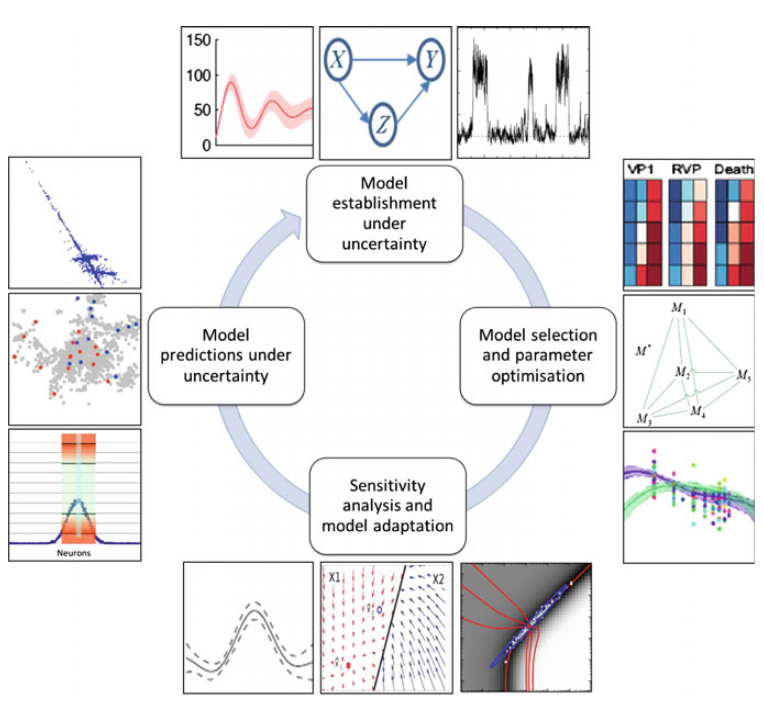
\includegraphics[width=0.8\textwidth]{images/model_cycle.png}
    \caption{Schematic overview of the model development life cycle under uncertainty: (i) establishment of a model under uncertainty, (ii) model selection and parameter optimization, (iii) sensitivity analysis and model adaptation, (iv) model predictions under uncertainty.  Reprinted from \cite{Uncertaintybiology}.}
    \label{fig:model_cycle}
\end{figure}
  
 A crucial part in model development is parameter estimation and optimisation. Statistically-driven parameter optimisation techniques: simulated annealing, genetic algorithms, particle swarm optimisation, etc. Global parameter search techniques include set inversion, constraint propagation techniques, and set-valued constraint propagation. Baysian approaches can be used for subsequent model assessment.
  
  Figure \ref{fig:model_cycle} showcases a life-cycle of typical model development under uncertainty. First, all uncertain parameters must be identified and, if relevant, structural uncertainties must also be included. Then, knowledge of the system can help select the most appropriate mathematical model for parameter optimization. This step can be assisted with UQ and SA techniques, by providing information on the most relevant parameter and which can be fixed to a nominal value before further analysis, as well as necessary changes in the model. Finally, several evaluations of the model are performed to produce model outputs incorporating model uncertainty.
 

  \section{Uncertainty quantification of multi-parameter models} \label{sec:UQ}
  
   The common way to assess model uncertainties is by treating the input factors as random variables, associated with a probability distribution, and performing several assessments of the model to estimate the uncertainty in the output responses.
   
    
Uncertainty quantification (UQ), or uncertainty analysis (UA), is a group of methods used to investigate the uncertainty in a model output that is generated from uncertainty in parameter inputs. The purpose of UQ is to quantify the degree of confidence in the values chosen for the model parameters, while it also allows to assess the reliability and sensitivity of complex  models. More broadly, UQ methods can be used to gain insight into how uncertainties propagate through the model and thus can help guide model verification and model improvement. UQ has been successfully applied to computational models across several engineering problems. 
  	
UQ can be applied in two main problems: forward uncertainty propagation analysis, and parameter sensitivity analysis.
 \textbf{Forward uncertainty propagation} analyses how uncertainties in the input parameters propagate through the model and affect the output  QOIs. In this framework, model parameters are treated as random variables with known probability distributions. This process is illustrated in Fig. \ref{fig:UQ_SA_framework}. When \textit{a priori} knowledge to estimate the probability distributions is lacking probability density functions (PDF) can be used to defined model uncertainties. PDFs for the QOIs can then be constructed by performing multiple simulations with parameters values sampled from the PDF, using a suitable sampling method. In this framework, the uncertainty  associated with the input variables can be propagated directly (forward) to the outputs via direct computation of the simulations. %SA will be discussed in the next section.
 
 \vspace{0.5cm}
 As mentioned in the introduction,  computational models are  often rather complex and may contain several hundreds of parameters that need to be calculated every iteration, and thus each single simulation can become quite  expensive computationally. Thus, it is desirable to be able to represent the overall behaviour of the model using a much more computationally tractable model. Therefore, in the UQ/SA framework it is often useful to analyse the workings of the model by replacing the model with a simpler ``surrogate'' model $f^{\prime} \approx f$), also referred to as \textit{metamodel}, which emulates the mapping of  input to output variables. The surrogate model chosen is often a function with well-defined behaviour, and used as a \textit{response surface} with high predictive capacity and low computational cost \cite{IOOSS20061241}. Polynomials, especially linear and quadratic functions, are common choices of metamodel, as well as splines, Gaussian processes, generalized linear models, among others. Quite often, these models are not able to emulate highly non-linear models with a sufficient level of predictive accuracy, and thus statistical learning models, such as support vector machines, and neural networks become preferable choices. 
 
 In order to define $f^{\prime}$, some \textit{a priori} knowledge of the system must be provided. When not enough \textit{a priori} knowledge exists to define $f^{\prime}$, it can be estimated by performing a ``large enough'' number of simulations with varying  parameters to infer relationships between model inputs and outputs. %Once the output spaces are known, different methods can be used to find mechanistic relationships between inputs and outputs, and thus build a surrogate model that allows to make predictions of the output from new input values. 
  The choice of a particular distribution will depend on \textit{a priori} knowledge and assumptions of the nature of the data.  When there is data characterizing the morphology of the uncertainty, this knowledge can be used to choose the most suitable probability distribution. However, when no prior knowledge is given about the nature of uncertainty, the best option is often to use the uniform distribution, since this makes the least number of assumptions on the likely of each particular value occurring. On the other hand, when it is known that values around the nominal value are more likely to occur, for instance from experimental data, then it is often more reasonable to assume a normal distribution. Some authors also argue that it is in general preferable to obtain the probability distribution of the uncertainty in the input parameters by specifying selected quantiles of the CDF, rather than using `standard' probability distribution \cite{HELTON20061175}. However, doing this often requires expert knowledge, and sometimes experimental measurements, and thus might be in some cases impractical.    Table \ref{tab:distributions} lists some of the commonly used probability distribution functions in UQ. 
  
  UQ results, i.e. the uncertainty in the output variables of a model, are usually presented are either statistical moments of the probability distribution, such as mean and variance, or as a reconstruction of the PDF, CDF, or even complementary CDF of the output uncertainty. Box plots can also be used to represent the output uncertainty, since they provide a compact and informative visualization of the probability distribution.

  
 %\begin{figure}[h]
  %	\centering
  	%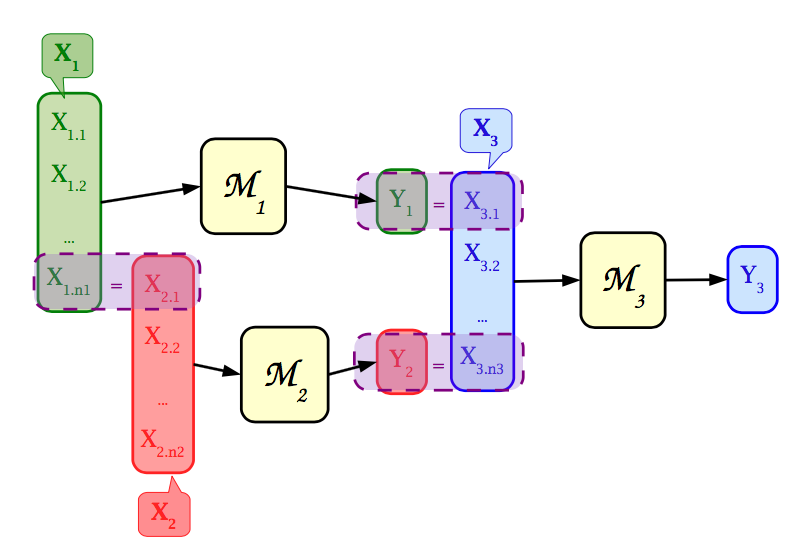
\includegraphics[width=0.7\textwidth]{images/Uncertainty_propagation.png}
  	%\caption{Illustration of uncertainty propagation in models with mutual input parameters. Reprinted from \cite{SudretPresentation}.}
  	%\label{fig:Uncertainty_propagation}
 % \end{figure}
  
    \begin{figure}[h]
  	\centering
  	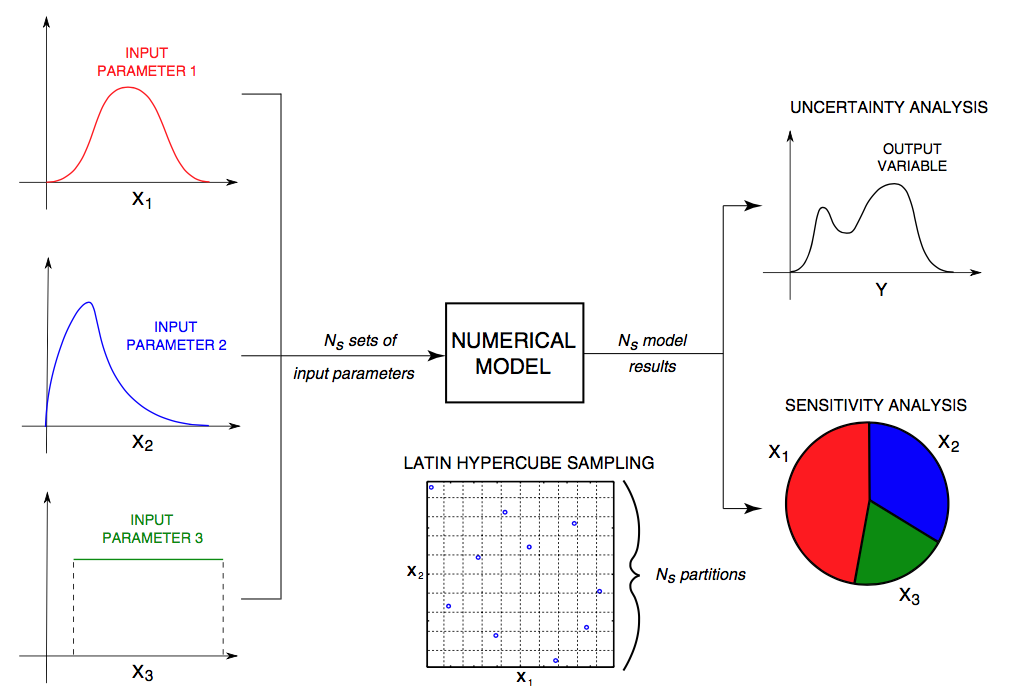
\includegraphics[width=0.9\textwidth]{images/UQ_SA_framework.png}
  	\caption{Reprinted from \cite{DEMICHIELIVITTURI201677}.}
  	\label{fig:UQ_SA_framework}
  \end{figure}
  
  \begin{table} 
  \begin{center}
  	\caption{Table of common probability distributions \cite{distributions}. }
  	\renewcommand{\arraystretch}{1.5}
  	\label{tab:distributions}
  \begin{tabular} {|c | l | c|} \hline
  	\textbf{Name} & \textbf{Probability density function}& \textbf{Representation} \\ \hline
 \rule{0pt}{25pt}Uniform & $f(x)=\frac{1}{b-a}, \hspace{1cm} a<x<b, -\infty<a<b<+\infty$ &  \begin{minipage}{3cm}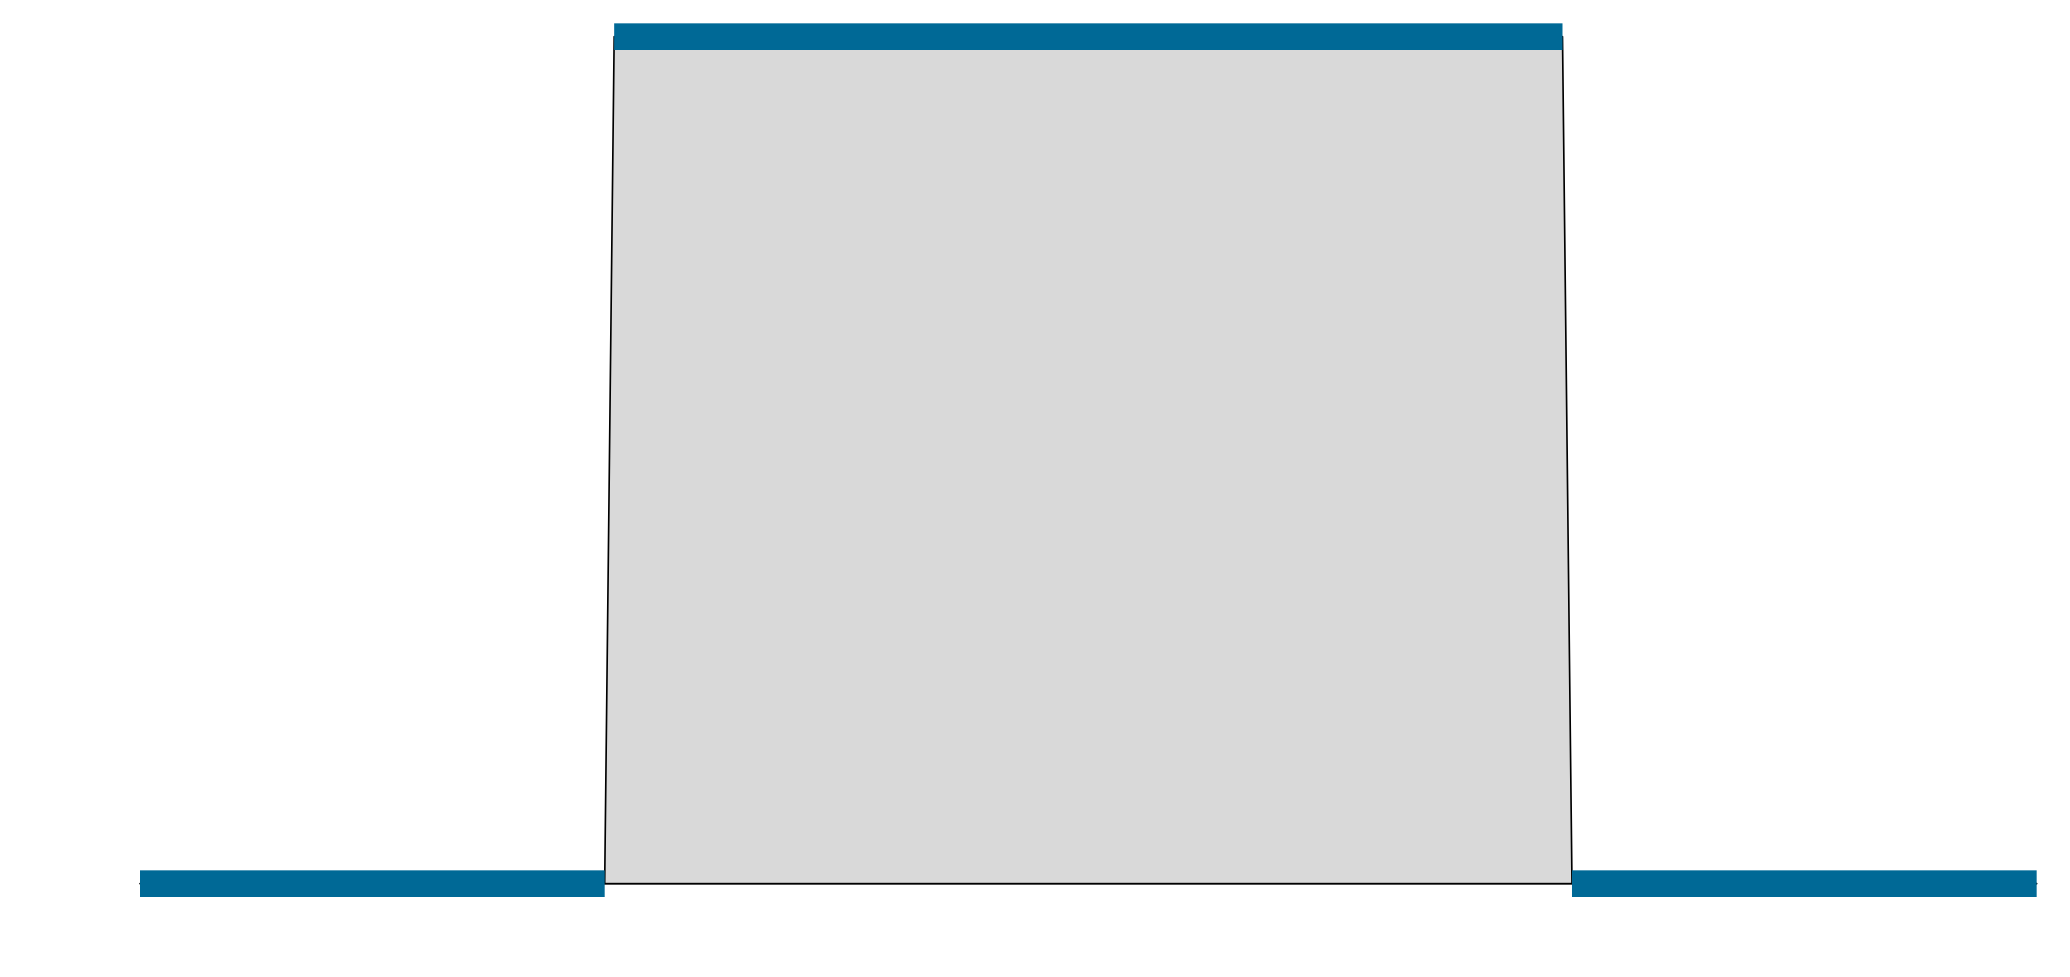
\includegraphics[width=1\textwidth]{images/uniform2.png} \end{minipage}  \\ \hline 
 
  \rule{0pt}{25pt} Normal &  $f(x)=\frac{1}{\sqrt{2\pi}\sigma}e^{-\frac{(x-\mu)^{2}}{2\sigma^{2}}}, \hspace{1cm } -\infty<x<+\infty$ & \begin{minipage}{3cm}\includegraphics[width=1\textwidth]{images/Normal_dist.png} \end{minipage}\\  \hline
  
  \rule{0pt}{25pt} Log normal & $f(x)=\frac{1}{x\beta\sqrt{2\pi}}e^{-\frac{1}{2}(ln(x/\alpha)/\beta)^{2}}, \hspace{1cm} x>0$ &  \begin{minipage}{3cm}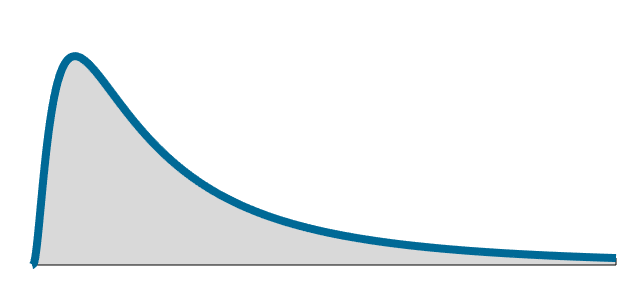
\includegraphics[width=1\textwidth]{/images/Lognormal_dist.png} \end{minipage} \\ \hline
 
  Triangular & $f(x)=
  \begin{cases}
  \frac{2(x-a)}{(b-a)(m-a)}, \hspace{1cm} a<x<m \\
  \frac{2(b-x)}{(b-a)(b-m)}, \hspace{1cm} m \geq x<b \\
  \end{cases}
  $ 
  & \begin{minipage}{3cm}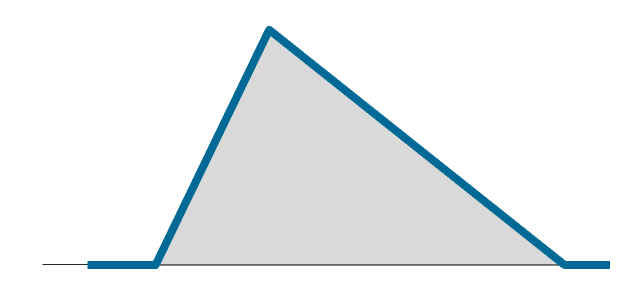
\includegraphics[width=1\textwidth]{images/Triangular_dist.png} \end{minipage}\\  \hline
  
  \rule{0pt}{25pt} Gamma & $f(x)=\frac{x^{\beta-1}e^{-x/\alpha}}{\alpha^{\beta}\Gamma(\beta)}, \hspace{1cm} x>0$ & \begin{minipage}{3cm}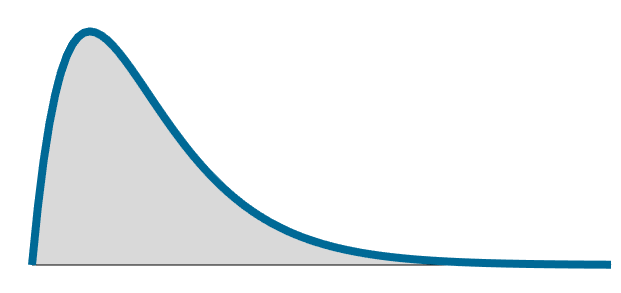
\includegraphics[width=1\textwidth]{images/Gamma_dist.png} \end{minipage} \\  \hline
  
 \rule{0pt}{25pt} Logistic & $f(x)=\frac{\lambda^{\kappa}\kappa e^{\kappa x}}{(1+(\lambda e^{x})^{\kappa})^{2}}, \hspace{1cm} -\infty<x<+\infty$ &  \begin{minipage}{3cm}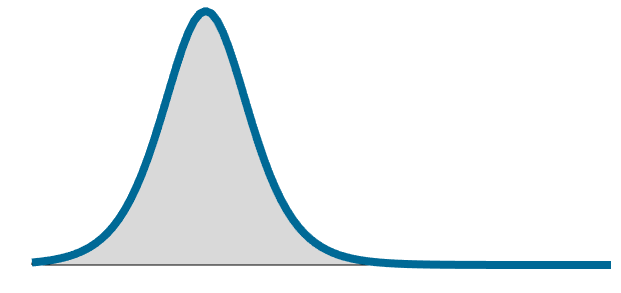
\includegraphics[width=1\textwidth]{images/Logistic_dist.png} \end{minipage}\\ \hline
  
  Laplace & $f(x)=
  \begin{cases}
  (1/(\alpha_{1}+\alpha_{12}))e^{x/\alpha_{11}}, \hspace{1cm} x<0\\
  (1/(\alpha_{1}+\alpha_{12}))e^{-x/\alpha_{11}}, \hspace{1cm} x \geq 0\\
  \end{cases}
  $& \begin{minipage}{3cm}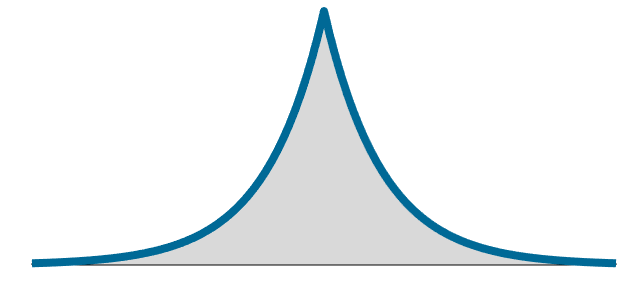
\includegraphics[width=1\textwidth]{images/Laplace_dist.png} \end{minipage} \\ \hline
  
    \rule{0pt}{25pt} Poisson & $f(x)=\frac{\mu^{x}e^{-\mu}}{x!}, \hspace{1cm} x=0,1,2,...$ & \begin{minipage}{3cm}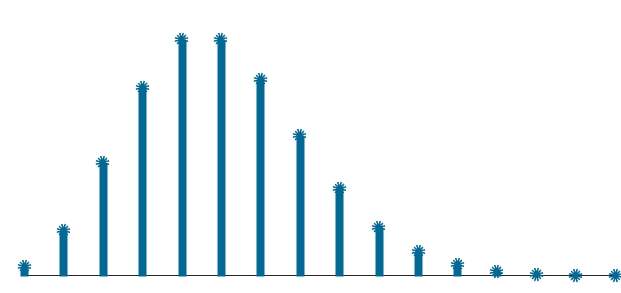
\includegraphics[width=1\textwidth]{images/Poisson_dist.png} \end{minipage}
    
    \\  \hline
    
  \end{tabular}
\end{center}
\end{table}

  \subsection{Monte Carlo sampling}
  
 Monte Carlo (MC) methods refer to a class of techniques of statistical sampling used to approximate solutions to problems without closed-form solution. An MC simulation consists of performing multiple model evaluations using random (or pseudo-random) sampling of probability distributions of model inputs. The MC method was initially formulated to estimate the integral of functions where it could not be determined analytically. 
 
 Each input parameter of the model is sampled from a specific of a probability distribution, depending on existing data and \textit{a priori} information. If there are no available data, a natural choice is a uniform distribution (with a large enough range with minimum and maximum values for the parameters that covers the parameter space). If knowledge of the system exists that suggests a more frequent or expected value for a particular parameter, a common option would be to use a normal distribution with a large enough variance.
  
  Typically, Monte Carlo (MC) methods are used as standard approach for UQ thanks to their accuracy and ease of implementation. On the down side, MC method require a high number of samples to converge. In fact, the accuracy of UQ results with the MC method is inversely related to the square root of the number of simulations (with the full model) performed. For complex models, they are very computationally expensive and cumbersome.  
  
  The MC method is a common approach ti perform UQ due ot its simplicity and good statistical results. However, this method is computationally expensive, and thus other methods have been developed that make UQ of large models with several uncertain parameters more computationally tractable. Improved sampling methods, such as the Latin-Hypercube sampling, and stochastic spectral methods such as the Polynomial Chaos Expansion, stochastic collocation, and stochastic reduced order models, are attractive alternatives.

\subsection{Latin-hypercube sampling}

The Latin-Hypercube sampling (LHS) method is a particular case of the MC method. This algorithm was developed to address the problem of under-sampling of values in the outer ranges of the pdfs.  In this method, the input parameter space is partitioned into $n$ intervals of equal probability that are randomly sampled.  It is based on a technique called \textit{stratified sampling without replacement}. Stratification divides the cummulative probability distribution curve into equal intervals; one sample is then randomly taken from each interval without replacement  so that the entire range for each parameter is explored and  thus faithfully recreating the input pdf. Therefore, LHS allows for an unbiased estimate of the variation in the model output while requiring fewer samples than the standard random sampling with the MC method. Furthermore, this sampling scheme allows to uncover any hidden correlations between parameters.

The LHS algorithm can be applied to any type of continuous probability distributions, but typically the normal and uniform distributions are used. An example of how the LHS algorithm partitions the cumulative pdf is represented in Fig. \ref{fig:LHS}.

\vspace{0.5cm}
\begin{figure}[h]
	\centering
	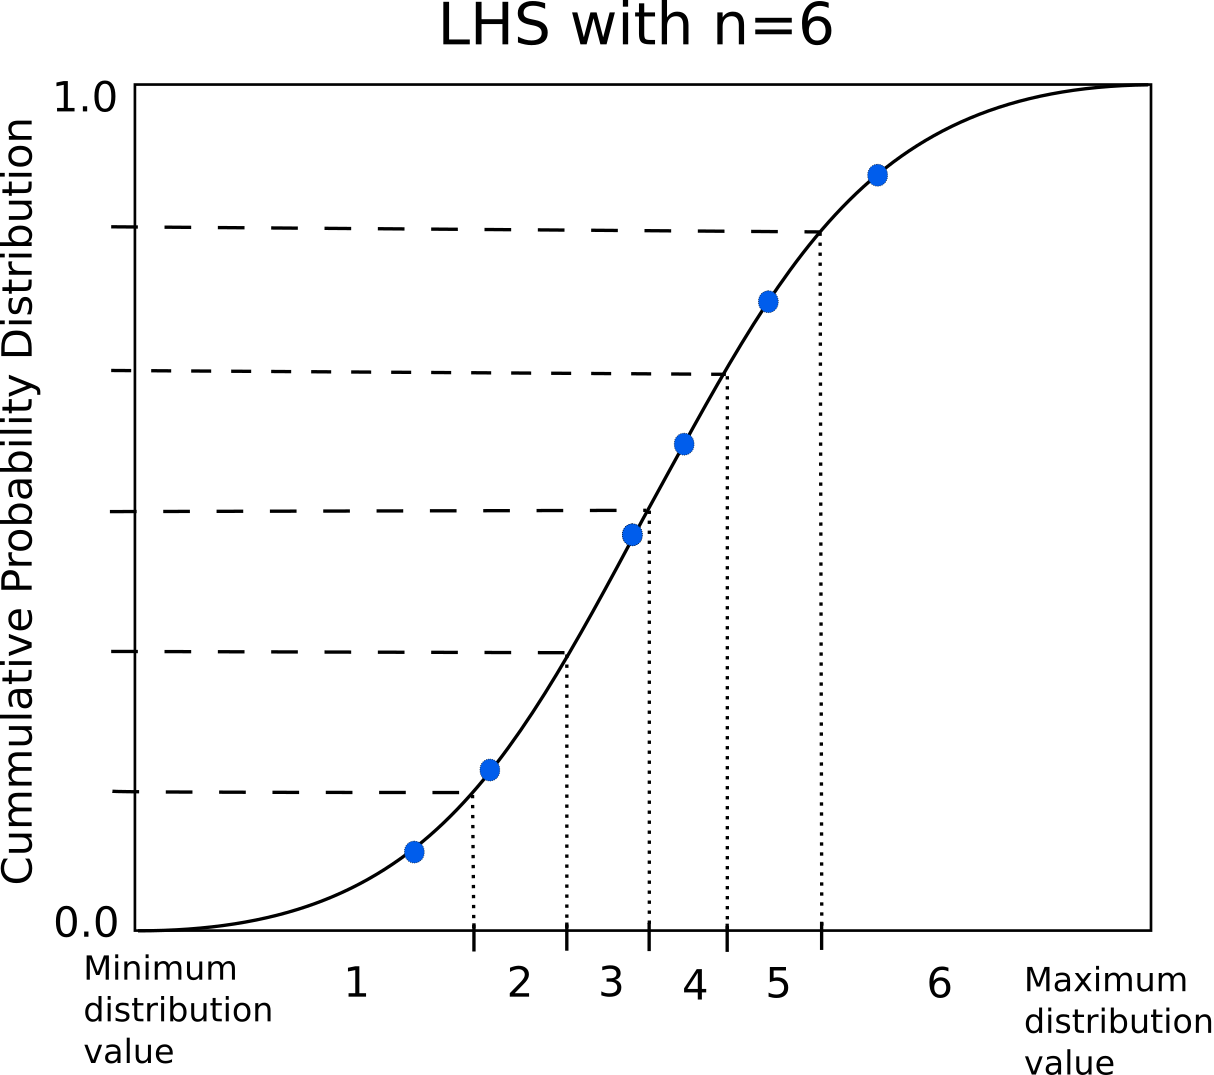
\includegraphics[width=0.5\textwidth]{images/LHS.png}
	\caption{Schematic representation of the LHS method of the cumulative distribution function.}
	\label{fig:LHS}
\end{figure}

  \subsection{Generalized Polynomial Chaos Expansion}
  
A common metamodelling approach is the so-called generalized polynomial chaos expansion (PCE). This method consists on building a response curve (\textit{surrogate model}) based on polynomial functions to replace a computationally expensive model and perform dimensionality reduction. It is a common method for performing UQ and global SA.
% which is based on a probabilistic framework.The main idea behind PCE is to replace a computationally expensive model with a surrogate model, also called response surface,  which is more computationally tractable for new input values. 

In generalized PCE, a given variable is represented by means of second-order stochastic processes ($\hat f(w)$). The PCE is constructed with a truncated linear combination of polynomial basis functions. Each independent variable is replaced by a parametric equation i $w$. Thus, the expansion can be written as:

%\begin{equation}
%%y(x,t,\xi) \approx \displaystyle\sum_{k=0}^{P}  \beta_{k}(x,t)\Psi_{k}(\xi)
%\hat f(x)=\sum^{N}_{n=0}C_{n}\Phi_{n}(x)
%\end{equation}

\begin{equation}
%y(x,t,\xi) \approx \displaystyle\sum_{k=0}^{P}  \beta_{k}(x,t)\Psi_{k}(\xi)
\hat f(w)=\sum^{P}_{k=0}C_{k}\Phi_{k}(\mathbf{\xi}(w))
\end{equation}
%\[\mathbf{X}=(X_{0}, X_{1},\cdots,X_{P})\]

Where $\Phi_{k}(\mathbf{\xi}(w))$ are orthogonal polynomials of $\mathbf{\xi}$ of order $P$, and $\mathbf{\xi}=(\xi_{1},\cdots,\xi_{1n})$ is a $n$-dimensional vector of Gaussian random variables with joint probability distribution  $\rho(\xi)$, and $w \in \Omega$ is a random event. %, and with defined probability density $\rho$ in $\Omega$; 
The polynomial basis $\{\Phi_{k}\}$ must satisfy the orthogonality criterion $\langle \Phi_{i},\Phi_{j} \rangle=0$. The number of terms $P$ can be determined from the  order of the expansion, and the number of random variables. 

\begin{equation}
	P+1=\frac{(n+p)!}{n!p!}
\end{equation}

Given the basis functions satisfy the orthogonality property, the PCE coefficients $C_{k}$  (or spectral modes of the expansion) can be written as:

%\begin{equation}
%C_{n}=\int^{}_{\Omega}\rho (x)\hat f(x)\Phi_{n}(x)dx
%\end{equation}

\begin{equation}
C_{k}=\int^{}_{\Omega}\hat f(\mathbf{\xi}) \rho (\mathbf{\xi})\Phi_{k}(\mathbf{\xi})d\mathbf{\xi}
\end{equation}

 %Since the polynomial basis are all orthogonal, the expectation of $\hat f(X)$ is given by the polynomial of order zero (fixed factor). 

The most challenging part in using the PCE method is to determine the coefficients of the expansion. There are two main classes of methods: intrusive, and non-intrusive. In intrusive methods, all dependent variables and random parameters in the governing equations are replaced with their polynomial chaos expansions; however, this is in general quite a demanding, time consuming task, requiring high computational cost. Therefore, intrusive methods are often not the preferred choice. 

On the other hand, non-intrusive methods obtain approximations of the polynomial coefficients without making any modifications to the deterministic code, and thus do not require any additional modelling effort. There are several different approaches to non-intrusive methods: sampling based (for instance, Monte Carlo), point collocation based, and quadrature methods. Sampling-based often make use of random (eg., Monte Carlo) or LHS to estimate the above integrals. Given the complexity of these methods, here I will only focus on the Point Collocation (PC) method. For a complete review on other methods to solve the polynomial expansions, refer to \cite{HELTON20061175,Wiener}.

The non-intrusive PC method consists of choosing an appropriate function basis ($\Phi_{k}(\mathbf{\xi}$ terms) to construct the response surface. Then, $N_{P}$ random point vectors in the input space, and performing model evaluations for each of the random points. These will provide $N_{P}$ estimations ($ \hat f(\xi_{n})$) of the response surface; typically, $N_{P} > (P+1)$. These can then be replaced in of eq. \ref{eq:PCEsystem}, yielding a system of linear equations, where the only unknowns are the spectral modes, $ C_{P}$. If the system is over-determined (case in which there are more collocation points than polynomial terms), then the linear system can be solved with the Least Squares method. 
 
  \begin{equation}
 \label{eq:PCEsystem}
 \begin{bmatrix} 
 \Phi_{0}(\xi_{0}) &  \Phi_{1}(\xi_{0}) & \dots &  \Phi_{P}(\xi_{0}) \\
 \Phi_{0}(\xi_{1}) &  \Phi_{1}(\xi_{1}) & \dots &  \Phi_{P}(\xi_{1}) \\
 \vdots & \vdots & \ddots & \vdots \\
 \Phi_{0}(\xi_{n}) &  \Phi_{1}(\xi_{n}) & \dots &  \Phi_{P}(\xi_{n}) \\
 \end{bmatrix}
 \times
 \begin{bmatrix}
 C_{0} \\
 C_{1} \\
 \vdots \\
 C_{P} \\
 \end{bmatrix}
 =
 \begin{bmatrix}
 \hat f(\xi_{0}) \\
 \hat f(\xi_{1}) \\
 \vdots \\
 \hat f(\xi_{n}) \\
 \end{bmatrix} \\
 \end{equation}
 
 
%The PCE coefficients can be determined form na initial set of sample points $x=\{x_{1},\cdots,x_{N}\}$, and model solutions via direct computation with the full model $f(x)$. Once the process is defined, it can be used to make predictions. Monte Carlo simulations of the surrogate model. 

%Allows to estimate expectation and variance of the process y:

%\begin{equation}
%\begin{aligned}
%	E{y(x,t)}=\beta_{0}(x,t) \\
%	E{(y(x,t)-E{y(x,t)})^{2}}=\displaystyle\sum_{k=1}^{\infty}\beta_{k}^{2}(x,t)\parallel \Psi_{k}\parallel^{2}
%\end{aligned}
%\end{equation}

 % PC uses a set of orthogonal polynomials (with regard to the inner product) multiplied by coefficients to define the surrogate model. The surrogate model gives a probability distribution of the output. That is, the PC propagates uncertainty in the input variables, defined by probability distributions, through the model to the output. 
 \vspace{0.5cm}
Fig. \ref{fig:PCE} illustrates a response curve with the collocation points highlighted in black. The main advantages to using PCE is linked to its computational efficiency in performing multiple model evaluations and relatively cheap estimation of the expansion coefficients with methods like the Least Squares, making it therefore a very attractive method for UQ. 
Furthermore, the capability to tackle non-linearities in the model and to allow for different parameter distributions to be defined is another major advantage of PCE.  %They rely on robust calculation of stochastic moments, such as mean and variance. 
On the down side, they require PC processes to be defined, which can be a non-trivial task. 
  
  \begin{figure}[h]
  	\centering
  	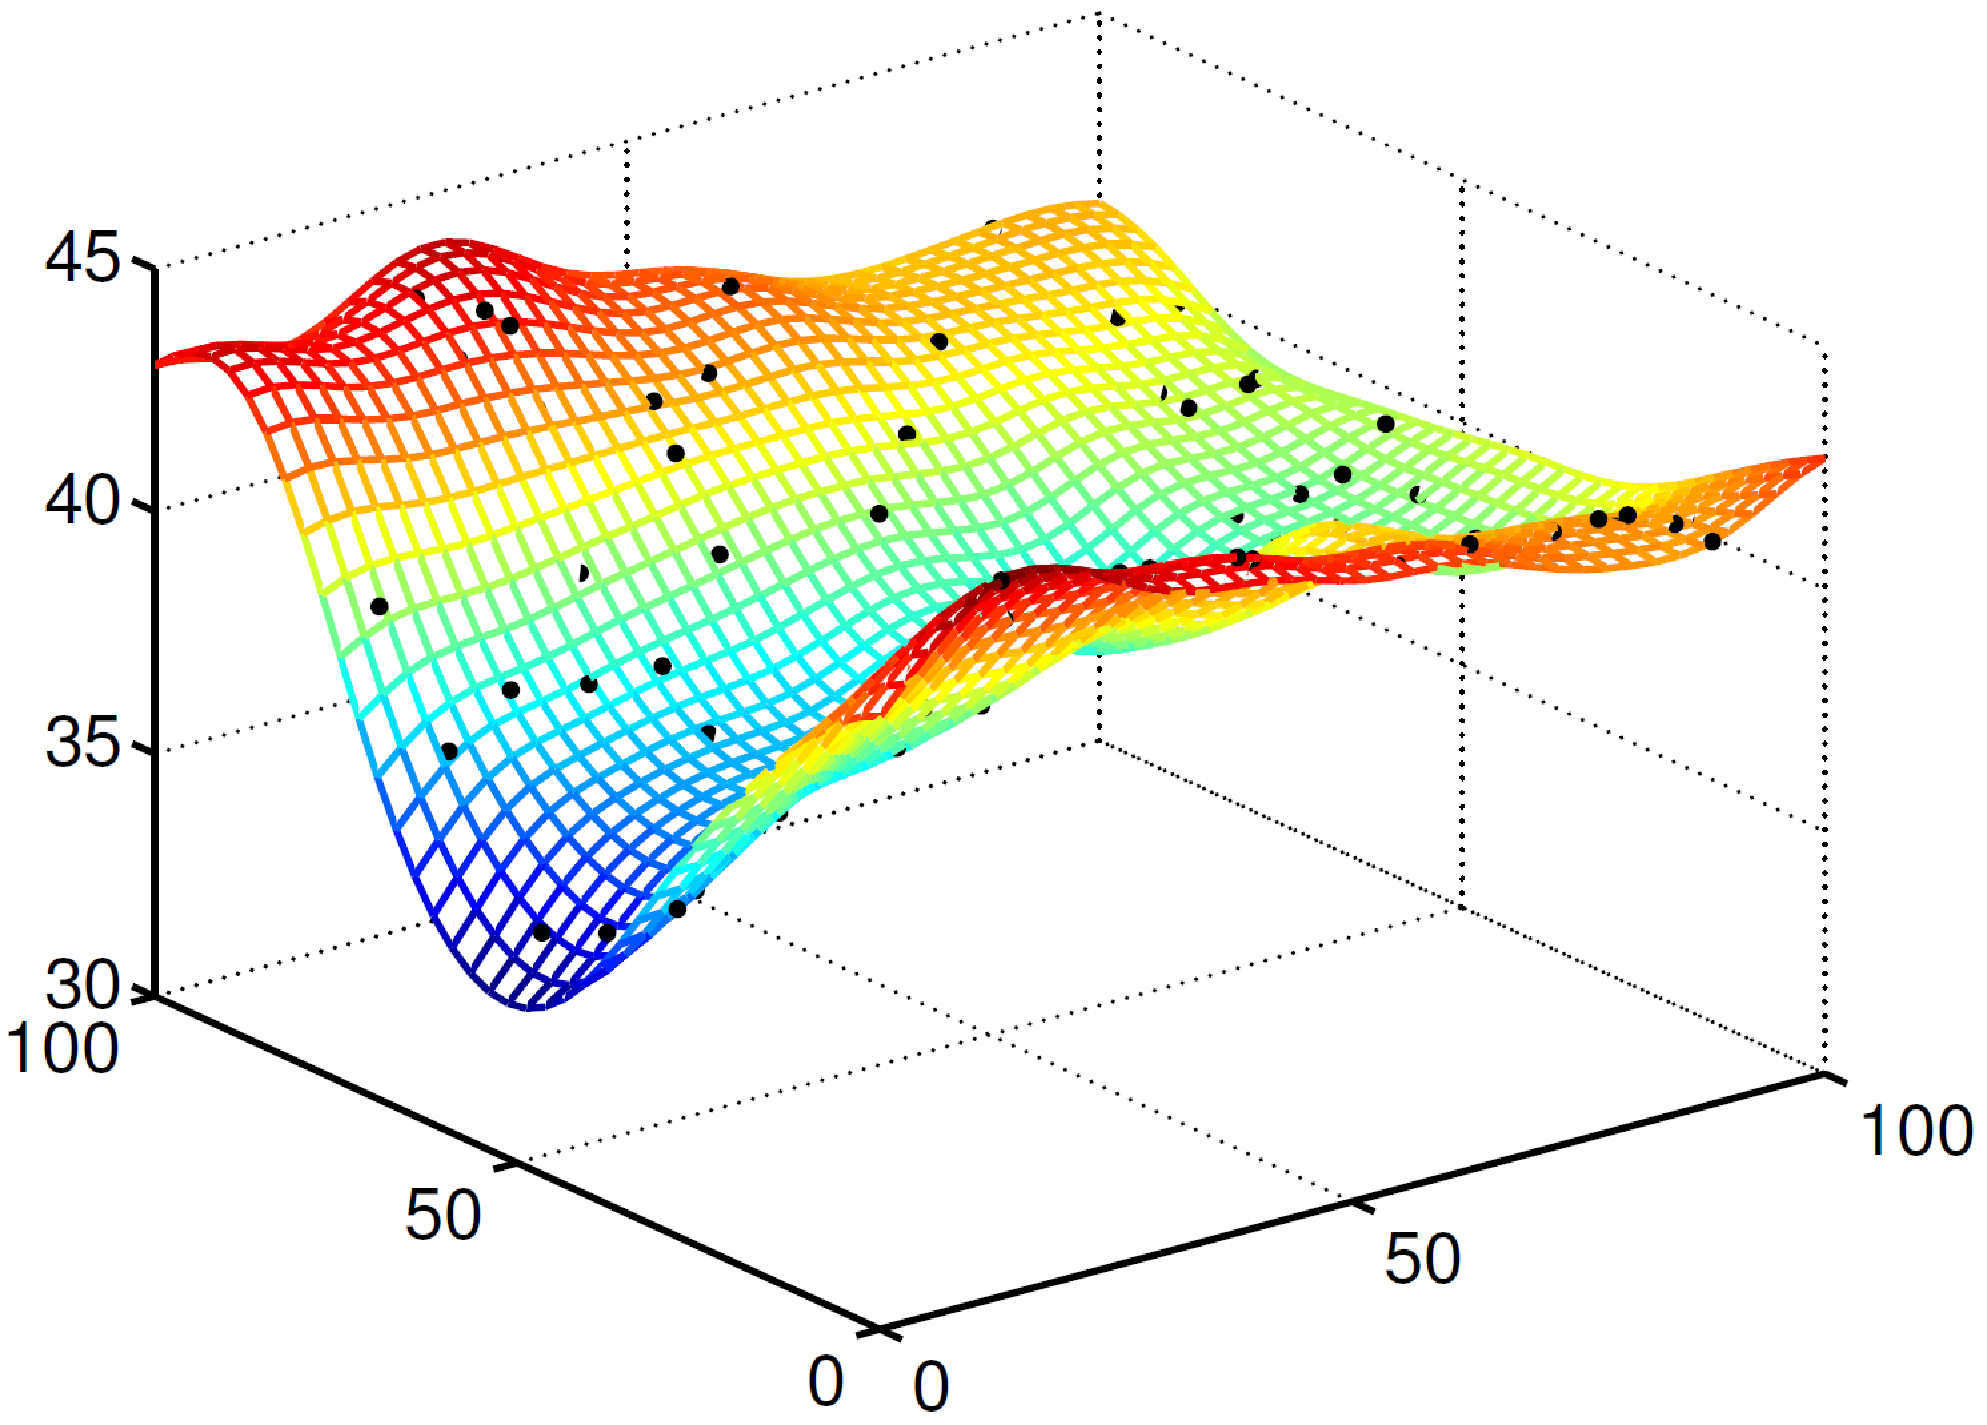
\includegraphics[width=0.6\textwidth]{images/Search_curve.png}
  	\caption{Representation of a search curve obtained with the Point Collocation method. Collocation points, shown in black, are used to perform evaluations of the model, which are then inserted into an over-determined system of linear equations to determine the PCE coefficients. Reprint from \cite{PCEfigure}.}
  	\label{fig:PCE}
  \end{figure}
  	

\section{Sensitivity analysis of multi-parameter models}

The purpose of sensitivity analysis is to measure how much the variation in input factors contributes to the variation observed in the model responses, that is, how ``influential'' a certain parameter is to the output. These measures are called \textbf{sensitivity indices} (SI). Sensitivity analysis has many applications in modelling,  as it allows: 
\begin{enumerate}
	\item to incorporate and understand the impact of uncertainty on model results
	\item  to do model optimization by prioritising the parameters are relevant for analysis, and fixing the others to their nominal values
	\item  to analyse model behaviour in comparison to other models
	\item to do model validation based on observations.  
\end{enumerate}
Thus, SA provides a framework for parameter identifiability, dimensionality reduction, and parameter constraint and optimization.  SA is a natural expansion of the UQ methods presented above, since it requires a large number of model simulations to be performed to obtained the distributions of the model responses, or quantities of interest (QOI). From these, relationships between model inputs and outputs, and among inputs, can be estimated to infer the role of the input parameters in the model. 

The choice of sensitivity analysis method depends on the nature of the input variables and of the responses. Several different approaches have been developed to extract \textit{importance measures} to estimate \textbf{sensitivity indices}. In a general way, the various methods have been classified as \textbf{screening methods}, \textbf{sampling-based}, \textbf{variance-based}, and \textbf{moment-independent SA}. 
SA encompasses a wide range of methods, so the purpose of this essay is not to give a comprehensive overview of all of the SA, but rather to give a brief insight into some of the main methods used. For a complete review of SA, refer to \cite{SaltelliThePrimer}. 


Additionally to the classification above, SA methods can also be divide into two categories: Local SA, and Global SA:

\textbf{Local sensitivity analysis (LSA)} $\rightarrow$ Explores the effect of small changes of model parameters  close to their nominal value; this is the preferred method when the input factors such as parameters or initial conditions are known with little uncertainty. The main approach is to examine the partial derivative of the response with respect to the input factors. 

\textbf{Global sensitivity analysis (GSA)} $\rightarrow$ parameters are varied simultaneously within a wide range, and variance in outputs correspond to the sum of variance in each input parameter individually plus covariance between input variables. 

\vspace{0.5cm}

Local methods for SA or one-at-a-time  (OAT) sensitivity analysis are the most commonly used methods due to their simplicity and ease of implementation, but they assume that model response to different inputs is independent. This assumption is quite often not true, and thus SA results can be biased. Global SA methods overcome this limitation by varying the input parameters simultaneously, thus quantifying the sensitivity of to that input by averaging the output over the other input parameters. The drawback is that GSA are more computationally costly and can become infeasible for expensive models. However, GSA that use a statistical emulator in place of the model (for instance, the Sobol method and FAST) can greatly reduce the computational cost of SA by requiring fewer model runs. 

Additionally, SA methods can  be subdivided into three broad classes: \textit{sampling-based}, \textit{variance-based}, and \textit{screening} methods. The sampling-based methods rely on the construction of a dataset of input and output pairs of values, in order to quantity relationships between the two groups. Examples of sampling-based SA methods include multi-parameter sensitivity analysis, regression models, and correlation analysis. In contrast, variance-based methods infer the sensitivities of the model based on decomposition of the output variance in components attributable to each input variables. Methods in this category include the Sobol Indices, and the Fourier Amplitude Sensitivity Test. The screening methods lie in between local and global SA since they scan the whole parameter space (so they are global in a sense), but using local derivatives to estimate the average effect of one variable at a time.

The particular effect of the variable to be quantified also varies with the SA method. \textit{Partial} sensitivity indices are based on importance measures that quantify only the marginal effect of an input variable on the outcome, that is the effect of varying that input alone. In contrast, \textit{total} sensitivity indices measure the combined marginal effect and interactions with other inputs on the variance of the output. 

%There exist several different methods for quantifying the sensitivities of model outputs to model inputs. 
SA techniques will perform differently for different types of computational problems. The choice of particular SA method mostly depends on the nature of the underlying model (non-linearities, monotonicity, and interactions among input variables), the structure of the data (continuous, sparse, binominal), and the desired sensitivity effect (partial versus total sensitivities). 

Another aspect of SA is the analysis of the evolution of sensitivity indices in time. This is called \textbf{dynamical}, or \textbf{time-varying SA}. I will not cover this in the present essay, but the basic idea behind dynamical SA is that in models with a time dependent component, the importance of the various parameters to the model output may vary over the time scale. When dealing with narrow time spans, sensitivities may be invariant in time and so checking SI in various time points might be unnecessary. However, if time-varying sensitivities have cannot be disregarded, sensitivities should be taken at different time points. If no \textit{a priori} knowledge exists on which are the critical time points to do the analysis, SA can be done in an exploratory way by performing multiple analyses at regular time intervals and checking for any time dependencies.

\vspace{0.5cm	}
The next subsections will give an overview of four SA methods commonly used in multi-parameter models. It is not meant to give an exhaustive description of all SA methods available. For further reading on sensitivity analysis methods and reviews, see \cite{SaltelliThePrimer, iooss:hal-00975701, HELTON20061175,Saltelli2000,SaltelliGuide}.

\subsection{Local SA with Partial Derivatives}

The Local Partial Derivatives method is a method of local SA that quantifies fluctuations in the model output due to the effect small perturbations in the input parameters \cite{Turanyi1990}. Typically, model parameters are varied one-at-a-time in a small degree, eg., 0.1 \%, while all the other input factors are fixed at their nominal values. Local sensitivity indices are quantified by first-order partial derivatives of the model output are taken with respect to the individual input variables. 

Partial derivatives measure the change in the slope of the tangent to the point $(\mathbf{x},f(\mathbf{x}))$ in the direction of $x^{0}_{i}$, fixing the remaining inputs, and thus do not take into account the effects of interactions among input factors. Therefore, global methods have been introduced to overcome this limitation.  
Additionally, since the sensitivities provided by the local method consider only the effects of variability in input parameters in a small range around their nominal values, this method is not suitable for performing SA in models with non-linearities and largely varying input parameters.
For a model of $N$ input variables:

\begin{equation}
  y=f(x_{1}, x_{2}, ..., x_{N})=f(\mathbf{x}),
\end{equation}

where $\{x_{1}, x_{2}, ..., x_{N}\}$ is a vector of $N$ independent parameters with nominal values $\tilde x=\{\tilde x_{1},\tilde x_{2}, ...,\tilde x_{N}\}$, the sensitivity index of  is given by the partial derivatives:

\begin{equation}
  S_{i}=\pdv{f(\tilde x)}{x_{i}}, %\frac{\delta}{\delta x_{i}}f(\tilde x)
\end{equation}

where $S_{i}$ is the sensitivity index of the $i$th input parameter, and measures how much changing $x_{i}$ influences the model output.

Since different input parameters can be expressed in different units and differ by several orders of magnitude, it is common to normalize the sensitivity indices. The normalization can be done with respect to either the mean value, the standard deviation, or as a percentage of parameter change:

\begin{equation}
\text{Mean value: }S_{i}=\frac{\tilde x_{i}}{f(\tilde x)}\pdv{f(\tilde x)}{x_{i}} %\frac{\delta}{\delta x_{i}}f(\tilde x)
\end{equation}
\begin{equation}
\text{Standard deviation: }S_{i}=\frac{\sigma(x_{i})}{\sigma(f(\tilde x))}\pdv{f(\tilde x)}{x_{i}} %\frac{\delta}{\delta x_{i}}f(\tilde x)
\end{equation}
\begin{equation}
\text{Percent change: }S_{i}=\frac{f(x_{1,...,x_{i}+p\%\cdot x_{i},...,x_{N}})}{p\%\cdot x_{i}}-\frac{f(x_{1,...,x_{i},...,x_{N}})}{p\%\cdot x_{i}}
\end{equation}

\vspace{0.5cm}
The main advantage of this method in comparison to global SA methods is its ease of implementation and low computational cost. Local SA can be use din the first stage of model development and analysis to obtain an overview of the model behaviour and pinpoint model inconsistencies. 

\subsection{The Morris Method}

The Morris method, or Elementary Effects method, is the most used screening method in sensitivity analysis \cite{Morris1991}. This method is used to identify non-influential variables in a model with a large number of variables. It uses a one-at-a-time (OAT) approach, whereby each input parameter is varied at once, thus allowing to quantify the main effects of varying each input individually. Like other screening methods, the Morris method provides quantitative measures of the sensitivities of the model, allowing to rank the inputs in order of importance. However, unlike other methods, this method does not allow to quantify the relative importance of the input variables. 

Consider the model $Y=f(X_{1}, X_{2}, \cdots, X_{k})$. In this method, the input space is discretized into a $k$-dimensional grid with $n$ levels. In each OAT analysis, a random trajectory in the input space is defined by randomly sampling the input space in a random direction of variation. Each trajectory has $(k+1)$ points where inputs are varied in steps $\Delta=\{0, 1/(p-1), 1/(p-1), \cdots, 1\}$, as illustrated in Fig. \ref{fig:Morris}. Each trajectory provides an estimate of the \textit{elementary effect} of each variable $X_{j}$ on $Y$, $E_{j}$. 

 \begin{figure}[h]
	\centering
	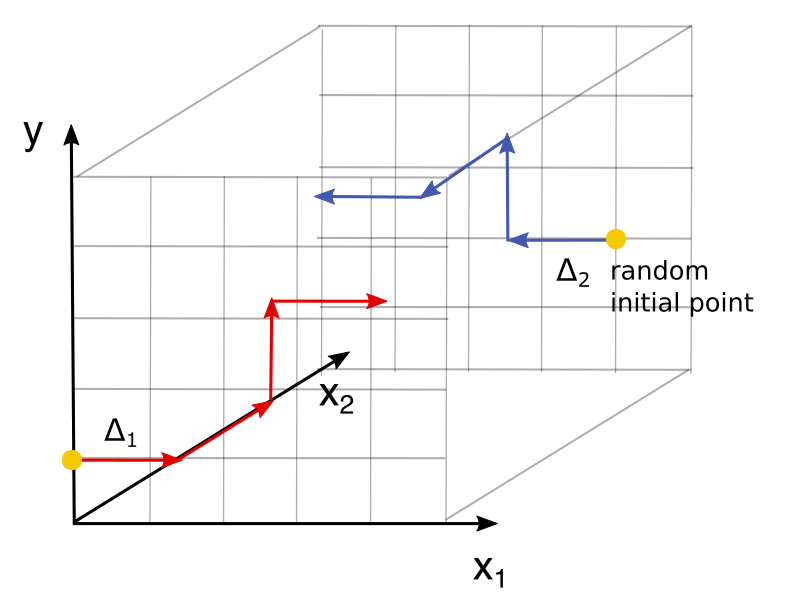
\includegraphics[width=0.5\textwidth]{images/Morris.png}
	\caption{Schematic representation of the Morris method, showing two different trajectories (red and blue) starting from different initial random points $(x_{1},x_{2})$.}
	\label{fig:Morris}
\end{figure}

\begin{equation}
E^{(i)}_{j}=\frac{f(X_{1},\cdots,X_{i-1}, X_{i}+\Delta,X_{i+1},\cdots,X_{k})-f(\mathbf{X})}{\Delta}
\end{equation}

\vspace{0.5cm}
A number $r$ of OAT analyses is performed for each input to estimate two importance measures, $\mu_{j}$ and  $\sigma_{j}$:

\begin{equation}
\mu^{*}_{j}=\frac{1}{r}\sum^{r}_{i=1}|E^{(i)}_{j}|
\end{equation}

\begin{equation}
\sigma_{j}=\sqrt{\frac{1}{r}\sum^{r}_{i=1}\Big(E^{(i)}_{j}-\frac{1}{r}\sum^{r}_{i=1}E^{(i)}_{j}\Big)^{2}}
\end{equation}

\vspace{0.5cm}

$\mu^{*}_{j}$ measures the overall importance of the input $X_{j}$ on the model output $Y$, and $\sigma_{j}$ measures the non-linear and/or interaction effects of of the inputs. The use of the mean of the absolute values of the elementary effects, proposed by Campolongo et al. \cite{CAMPOLONGO20071509}, resolved the problem of compensatory effects with opposite signs in non-monotonic models. 
The relationship between the values of $\mu_{j}$, and  $\sigma_{j}$ allow to group the variables into three distinct groups: inputs with negligible effects (small $\mu_{j}$, and large $\sigma_{j}$); inputs with  large effects without interactions (large $\mu_{j}$, and small $\sigma_{j}$); and inputs with non-linear and/or interactions effects (large $\mu_{j}$, and large $\sigma_{j}$).

The Morris method is useful method for performing SA given its simplicity. It allows screening model with a large number of parameters, without requiring certain properties such as monotonicity or additivity. Furthermore, it provides a measure of the main effects of a variable, including to some extent the effects arising from interactions with other variables \cite{CAMPOLONGO20071509}. The main limitation is that the design proposed by Morris \cite{} consists on varying parameters one-at-a-time, and therefore similarly to the partial derivatives method, it does not provide a measure of the output sensitivity to an input taking averaged in relation to the effects of the remaining inputs.


\subsection{Regression analysis}

Global SA can be performed with classical regression methods. This is a sampling-based form of SA, in that both inputs and outputs have to be sampled in order to provide the raw data to fit a regression model. 

 Regression provides an algebraic representation of the relationship between multiple input variables $X_{i}$, and an output variable $y$. Thus, it is a form of predictive modelling which investigates the relationship between one or more independent variables (predictors), and a dependent variable (response). 

Regression methods essentially find the `best-fit' of a set of data points to some sort of mathematical relation, whether that is linear, polynomial, logarithmic, exponential, or any other function. More typically, linear regression is used for fitting a straight line through a set of data points (observations) using some goodness-of-fit criterion. The mathematical expression is defined by a set of regression coefficients which provide information on:

\begin{itemize}
	\item  the significance of relationships between dependent variable and independent variable;
	\item  the strength of impact of multiple independent variables on a dependent variable.
\end{itemize}

Given this, regression coefficients can be used to provide a qualitative measure of sensitivity indices of the model to the input parameters, and thus rank the inputs in order of their importance. There are several different regression models (linear, polynomial, logarithmic, exponential, logistic etc.), and the particular choice of model depends on three main aspects: (i) the number of independent variables, (ii) the type of dependent variables, and (iii) the trends in the data. In Multiple Linear Regression (MLR), a straight line is fit to the data as a function of more than one independent variables. If several output variables are considered, it is called Multivariate Linear Regression (MVLR), or general Linear Model. I will be addressing only the cases of MLR and MVLR in the following subsection, as these have a broad range of applications.
%A tightly related concept to regression is that of correlation. Correlation provides a statistical measure of the relationship or association between the mean value of one variable and corresponding values of other variables, but not does fit a line through the data points. However, in some contexts these two concepts can be used interchangeably, as both the regression and correlation coefficients  provide a measure of the relation between the independent and the dependent variables of the regression model. More on correlation analysis is provided in the following subsection.




% Even though in most cases the output does not linearly depend on the input parameters, this approach has been shown to be a fairly good approximation of the true model, especially when perturbations of the system are small (ie, input parameters are varied in a tight range around their nominal value). 

\subsubsection{Multiple and Multivariate Linear Regression} \label{sec:MLR}

In most computational models a given response is influenced by more than one predictor. Therefore, it is often more useful to model the responses as a function of several predictors. This is called \textbf{Multiple Linear Regression (MLR)}. In MLR, each observation of the dependent variable $y_{j}$ can be expressed as a linear combination of the observed independent variables $x_{ij}$ and the regression coefficients $\beta_{ij}$, plus an intercept {$\beta_{0j}$ and a residual term $\epsilon$, much like in the simple linear regression model.
	
	\begin{equation}
	y_{j}  = \beta_{0} + \beta_{1}x_{j1}+\beta_{2}x_{j2}+\dots + \beta_{p}x_{jp} = \beta_{0} + \sum^{p}_{i=1} \beta_{p}x_{jp} + \epsilon\\
	\end{equation}

Where $p$ is the number of predictors of the linear model (or input parameters), and $y_{ij}$ is the $j^{th}$ response. % $\beta_{0}$ is the intercept term of the regression. 
The regression coefficients correspond to the slope of the line on the simple regression model. Typically, the number of independent observations of predictors and responses is much larger than the number of predictors. This ensures that the system is overdetermined and improves the prediction capacity of the model. 
In matrix notation, the model can be written as:

\[ \label{eq:MLR_model}
\begin{bmatrix} 
y_{1}  \\
y_{2}  \\
\vdots  \\
y_{n} \\
\end{bmatrix}
=
\begin{bmatrix} 
1 & x_{11} & x_{12} & \dots & x_{1p} \\
1 & x_{21} & x_{22} & \dots & x_{2p} \\
1 & \vdots & \vdots & \ddots & \vdots \\
1 & x_{n1} & x_{n2} & \dots & x_{np} \\
\end{bmatrix}
\times
\begin{bmatrix}
\beta_{0} \\
\beta_{1} \\
\vdots \\
\beta_{p} \\
\end{bmatrix}
+
\begin{bmatrix}
\epsilon_{1} \\
\epsilon_{2} \\
\vdots \\
\epsilon_{p} \\
\end{bmatrix}
\] 

\begin{equation} \label{eq:Linear_Regression1}
\mathbf{y} = \mathbf{X} \cdot \mathbf{\beta}+ \mathbf{\epsilon}
\end{equation}

\vspace{0.5cm}

where $p$ is the number of varied input parameters, and $\epsilon$ is the residual term of the model, which is assumed to have identical a normal distributions and be uncorrelated. Typically $n\gg p$ and $n\gg k$. In matrix representation, each independent observation of the predictors is a row in the $\mathbf{X}$ matrix, and each response (ie, the output of each individual simulation with the computational model) is an entry in the $\mathbf{y}$ vector.

%responses are arranged into a vector $y_{1,2,...,n}$, the responses into a matrix  $\mathbf{X}$ of predictors, and their corresponding output values into the output matrix $\mathbf{Y}$ of regressors. $\mathbf{y}$  can then be written as a linear function of  $\mathbf{x}$ with regression coefficients $\mathbf{\beta}$ plus a matrix of regression erros \textbf{$\epsilon$}. That is, for a particular output $y$, the MVLR can thus be written as:

% In matrix notation, each output $\hat y_{1,2,...,k}$ ($Y$)  can be expressed as a function of the product of the inputs $x_{1,2,...,p}$ ($X$) with the coefficients ($B$) . The solution of the system in respect to  $\mathbf{B}$ is an approximation of the regression coefficients, $\mathbf{\hat B}$, by minimizing $\epsilon$ (equation \ref{eq:Linear_Regression}). 

%In matrix notation,  the inputs into a matrix $x_{1,2,...,p}$ ($X$), and the coefficients ($B$) . The solution of the system in respect to  $\mathbf{B}$ is an approximation of the regression coefficients, $\mathbf{\hat B}$, by minimizing $\epsilon$ (equation \ref{eq:Linear_Regression}). 

In the case of the MVLR with multiple responses, the equations above can be written as:

\begin{equation}
y_{ij}=\beta_{0j}+\sum^{p}_{j=1}\beta_{ji}x_{ij}+\epsilon_{ij}
\end{equation}

 Similarly to MLR, here the outputs from each independent simulation constitute a single row in the $\mathbf{Y}$ matrix, and each column in the $\mathbf{B}$ matrix constrains the regression coefficients of the linear  model. The system can be written as: 

 \[
 \begin{bmatrix}
 y_{11} &  y_{12} & \dots &  y_{1k} \\
 y_{21} &   y_{22} & \dots & y_{2k} \\
 \vdots &  \vdots  & \ddots & \vdots \\
 y_{n1} &  y_{n2} & \dots & y_{nk} \\
 \end{bmatrix}
 =
\begin{bmatrix} 
1 & x_{11} & x_{12} & \dots & x_{1p} \\
1 & x_{21} & x_{12} & \dots & x_{2p} \\
1 & \vdots & \vdots & \ddots & \vdots \\
1 & x_{n1} & x_{n2} & \dots & x_{np} \\
\end{bmatrix}
\times
\begin{bmatrix} \label{eq:betas}
\beta_{01} & \dots & \beta_{0k} \\
\beta_{11} & \dots & \beta_{1k} \\
\vdots & \ddots & \vdots \\
\beta_{p1} & \dots & \beta_{pk} \\
\end{bmatrix}
+
\begin{bmatrix} 
\epsilon_{11} & \dots & \epsilon_{1k} \\
\epsilon_{21} & \dots & \epsilon_{2k} \\
\vdots & \ddots & \vdots \\
\epsilon_{n1} & \dots & \epsilon_{nk} \\
\end{bmatrix}
\]

\begin{equation} \label{eq:Linear_Regression2}
\mathbf{Y} = \mathbf{X} \cdot \mathbf{B} + \mathbf{E}
\end{equation}

where $n$ is the number of samples, $p$ is the number of varied input parameters, and $k$ is the number of outputs from the model. Again, the residuals random and are normally distributed with zero mean $(\epsilon_{i1}, ..., \epsilon_{ik}) \sim N(0,\Sigma)$.

Figure \ref{fig:Linear_model} schematically illustrates the typical dimensions of the data in MVLR of computational models with a large number of observations.

\begin{figure}[!ht]
	\centering
	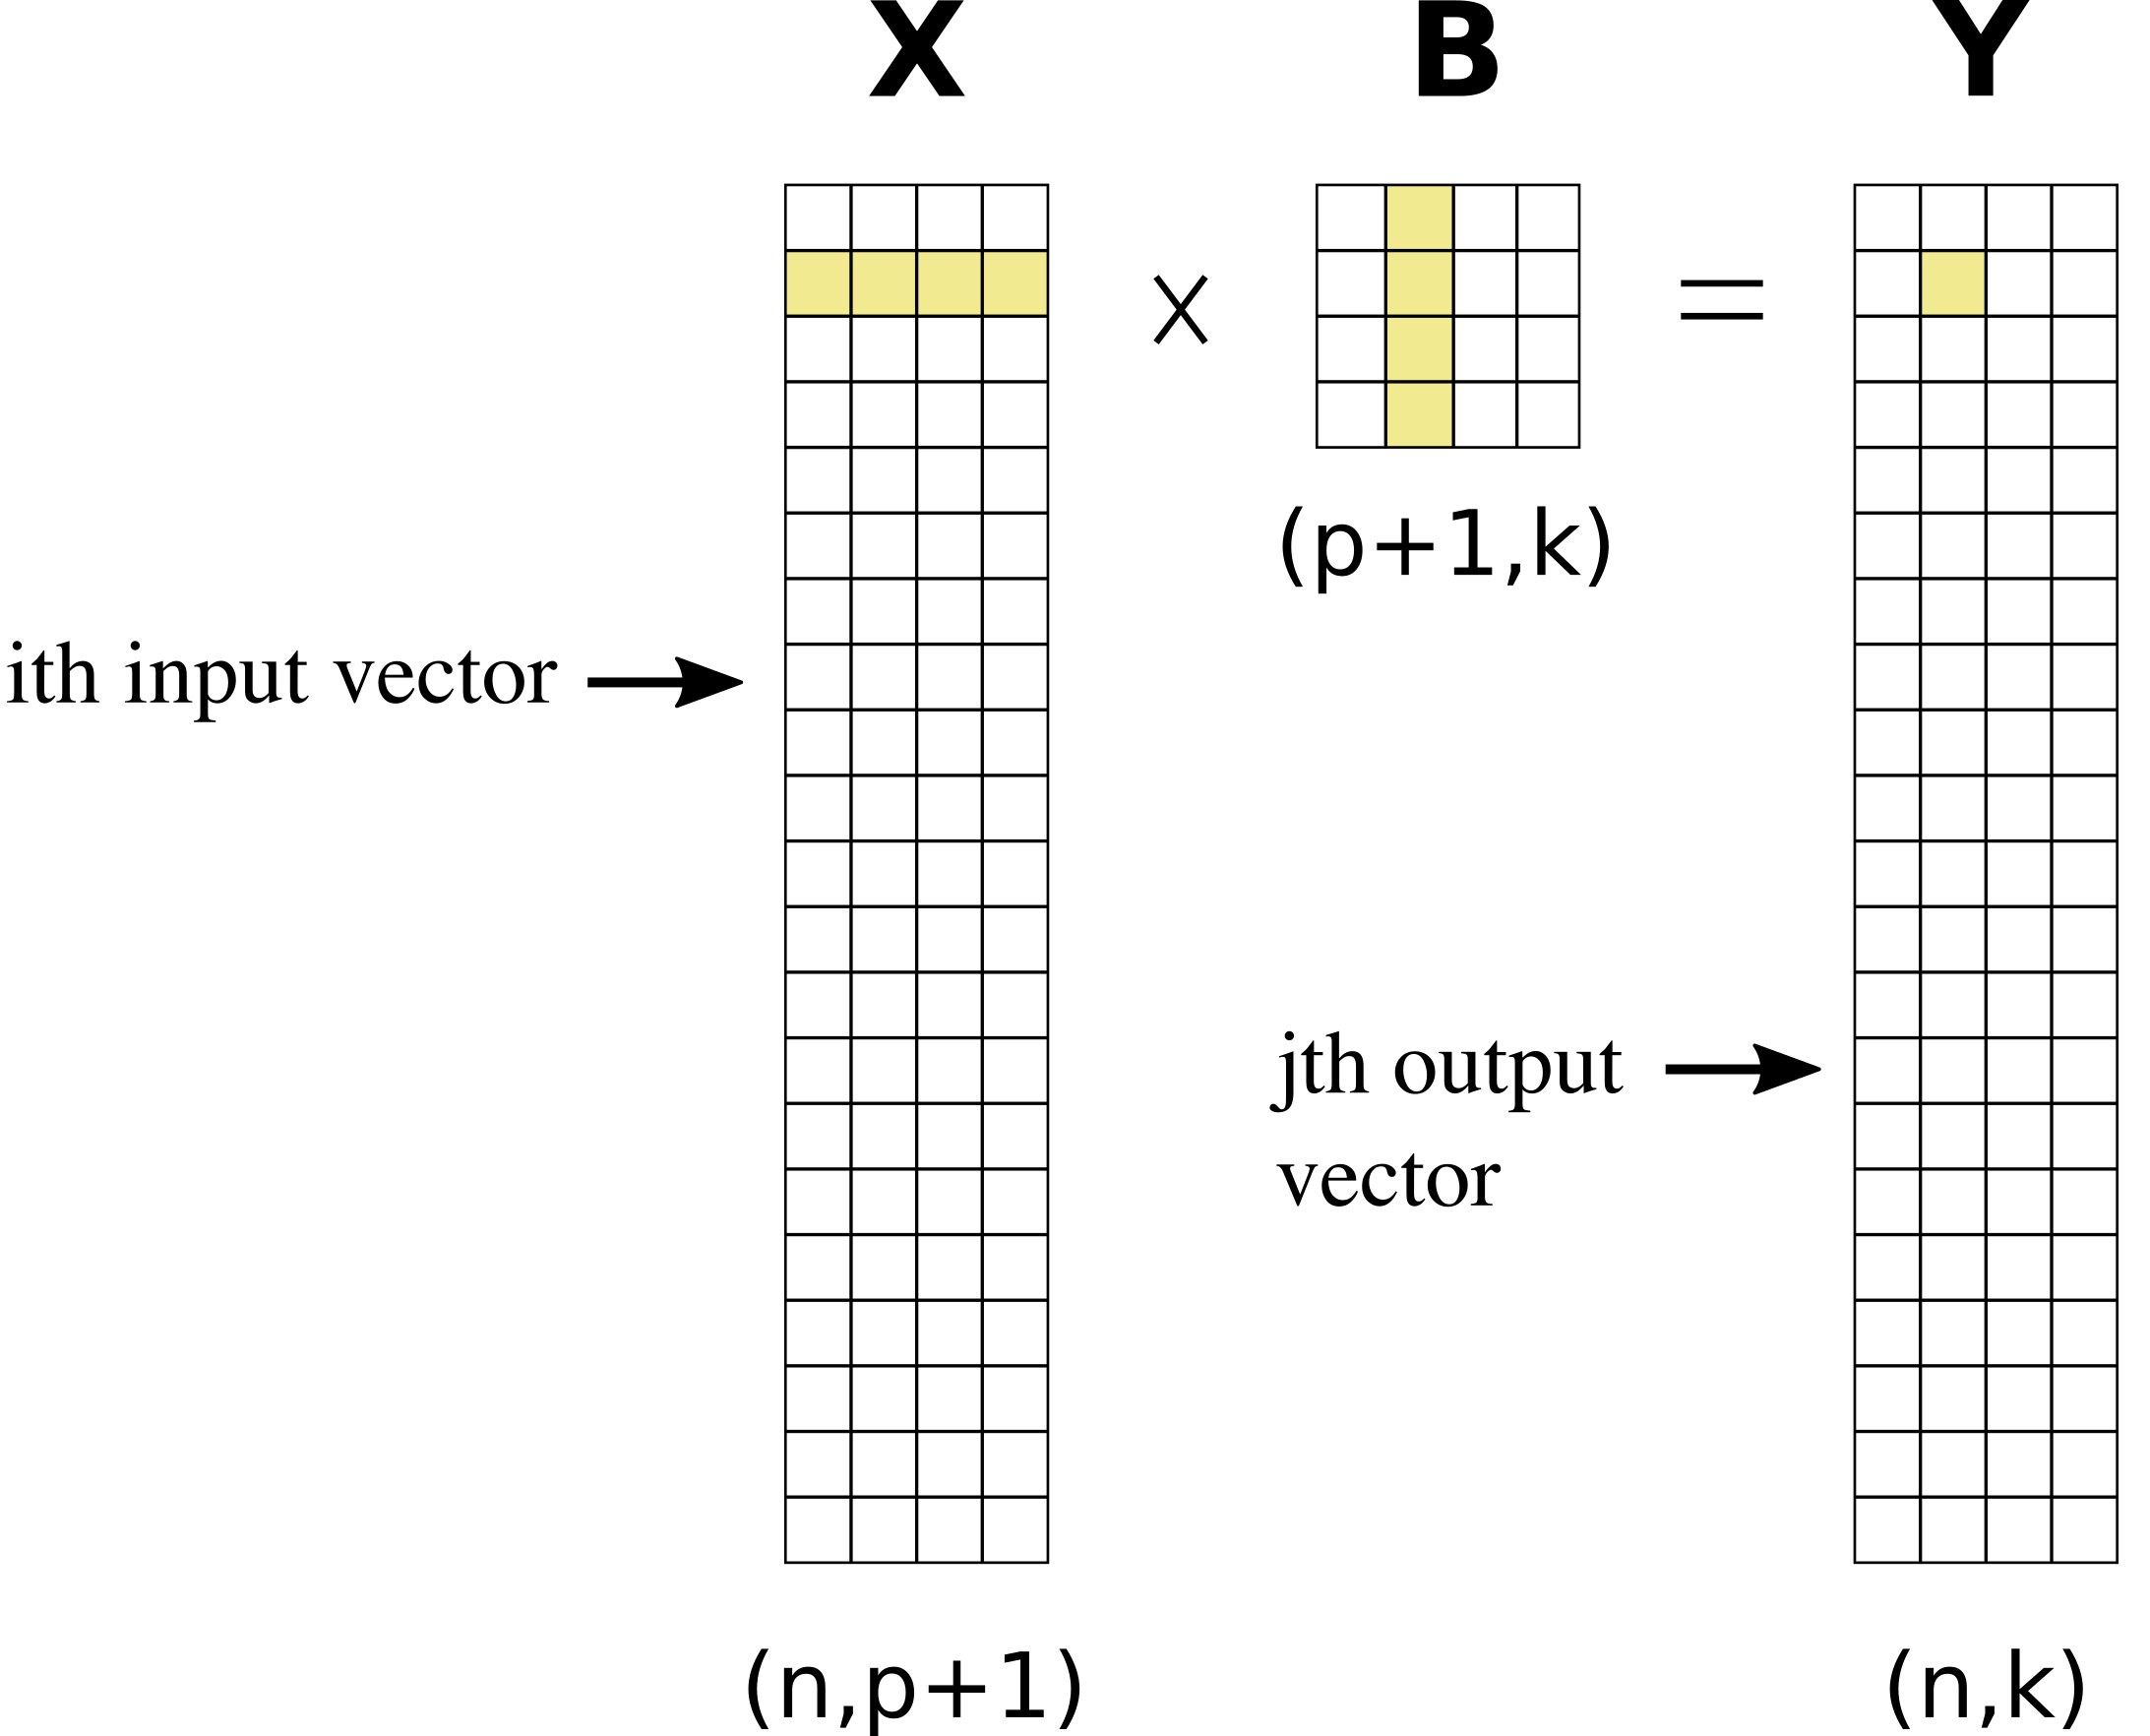
\includegraphics[width=0.5\textwidth]{images/Linear_model.png}
	\caption{Representation of the input and output data structure and in MVLR models.}
	\label{fig:Linear_model}
\end{figure}

In order to eliminate effects of different units among variables, regression coefficients are often expressed as normalized by the variances:
%An alternative way to obtain standard regression coefficients without the need to converting the variables to z-scores is to transform the $\beta_{j}$ by normalizing to the variance of the variables:

\begin{equation}
SRC_{j}=\hat \beta_{j}\sqrt{\frac{Var(X_{j})}{Var(Y)}}
\end{equation}

This is called the Standard Regression Coefficient (SRC). $SRC_{j}$ they measure the variable importance based on their effect on $y$ relative to $\text{Var}(y)$ of perturbing $X_{i}$ from $\mathbb{E}(X_{i})$ by a fixed fraction of $\text{Var}(X_{i})$. The larger the magnitude of $\beta_{i}$,  the more important is the input $X_{i}$ to the output $y$. A negative coefficient means that the independent and the dependent variables vary in opposite directions Importantly, the coefficients of regression in linear regression can only provide a \textit{quantitative} measure of sensitivities if the data is perfectly linearly related, that is, if the coefficient of determination of the regression (introduced in the next subsection) is approximately 1. Also, note that the SRCs provide  a useful measure of variable importance only if all the $X_{i}$ are independent, and they do not provide reliable indications otherwise.
. %\textcolor{red}{Below is an example of a representation of sensitivities of a model to several different input parameters.}

\subsubsection{Linear models with interaction terms}
The MVLR model can be expanded to include interaction terms between one or more predictor variables of order >1:

\begin{equation} \label{eq:interaction_terms}
y  = \beta_{0} + \sum^{p}_{j=1} \beta_{j}f_{k}(x_{1, x_{2}}, ...,x_{p}) + \epsilon\\
\end{equation}
\begin{equation} \label{eq:interaction_terms2}
\hat y  = \beta_{0} + \beta_{1}x_{1} + ... + \beta_{p}x_{p} + \beta_{p+1}x_{1}^{2}+ \beta_{p+2}x_{1}x_{2} + ...  \\
\end{equation}

Although a such a model is a polynomial model on $x$ of order 2, the model also can be seen as a linear combination of the $\beta$-parameters, with the $x$-terms being seen as the weights. Although the MVLR allows for a high degree of flexibility for the incorporation of interactions among variables, it is a highly complex process as it requires \textit{a priori} knowledge of the covariances of the independent variables. There are techniques that can assist in uncovering hidden relationships between input variables, but in many cases these interactions terms can be neglected with significantly compromising the accuracy of the predictions.

\subsubsection{Least Squares Regression}

The method of least squares is the most common approach in regression analysis to approximate the solution of overdetermined systems. This method is also often referred to as Least Squares regression. It allows to determine unbiased estimates of the $\beta$, often termed as least squares estimators ($\hat \beta$): 
	
    \begin{equation} \label{eq:OLS} 
	\mathbf{\hat y} = \mathbf{X} \cdot \mathbf{\hat \beta} %+ \epsilon \rightarrow  \hat{Y} = X \cdot B
	\end{equation}
		
	%\begin{equation} \label{eq:OLS} 
	%\mathbf{\hat Y} = \mathbf{X} \cdot \mathbf{\hat B} %+ \epsilon \rightarrow  \hat{Y} = X \cdot B
	%\end{equation}
	
When used with a linear regression model, it is called Ordinary Least Squares (OLS). The OLS fits a hyperplane into a $(p+1)$-dimensional space that minimizes the sum of squared residuals. "Least squares" means that the overall solution minimizes the sum of the squares of the residuals of the analytical and the predicted solutions. 
	
	The residuals are defined as:
    \begin{equation} \label{eq:residuals}
    \epsilon=\mathbf{y} - \mathbf{X}\beta = \mathbf{y} - \mathbf{\hat y}
	\end{equation}
	
	Thus, the sum of squared residuals is given by:

	
	\begin{equation}
	 \sum^{n}_{i=1}  \epsilon^{2}_{i} = \epsilon'\epsilon = (\mathbf{y} - \mathbf{X}\hat \beta)'(\mathbf{y} - \mathbf{X}\hat \beta)
	\end{equation}
	
	Thus, the problem can be formulated as:
	
	\begin{equation}
	\min_{\beta \in \Re^{p+1}}  \| \mathbf{y}-\mathbf{X}\beta \|^{2} = \min_{\beta \in \Re^{p+1}} \sum^{n}_{i=1}(y_{i}-\beta_{0}-\sum^{p}_{j=1}\beta_{j}x_{ij})^{2}
	\end{equation}
	
\vspace{0.5cm}
By the Orthogonal Decomposition Theorem, the residuals are minimal when $\epsilon_{i}$ are orthogonal to the columns of $\mathbf{X}$, resulting in a closed-form expression for calculating the $\hat \beta$:
	\begin{equation} \label{eq:betas2}
    \mathbf{X}'(\mathbf{y - \mathbf{X}\hat \beta}) = 0 \\ 
    \Leftrightarrow \hat \beta = (\mathbf{X}' \mathbf{X})^{-1}\mathbf{X}'\mathbf{y}
    \end{equation}

Which has a unique solution if the inverse of $(\mathbf{X}' \mathbf{X})$ exists, that is, if the columns of $\mathbf{X}$ are linearly independent (the predictors are all uncorrelated). In the case of MVLR, the OLS problem has the  same solution, where $\mathbf{\hat \beta}$ and $\mathbf{y}$ are replaced by the multivariate matrices:

\begin{equation} \label{eq:betas3}
 \mathbf{\hat B} = (\mathbf{X}' \mathbf{X})^{-1}\mathbf{X}'\mathbf{Y}
 \Rightarrow \hat \beta_{j} = (\mathbf{X}' \mathbf{X})^{-1}\mathbf{X}'\mathbf{y_{j}}
\end{equation}

%For the simple case the univariate regression, the expressions for calculating the regression coefficients $\beta_{1}$ and $\beta_{0}$ are given by:

%\begin{equation}
%\beta_{1} = \frac{\sum^{n}_{i=1}(x_{i}-\bar x)(y_{i}-\bar y)}{\sum^{n}_{i=1}(x_{i}-\bar x)^{2}}, \hspace{1cm} \beta_{0} = \bar y - %\beta_{1} \bar x
%\end{equation}

\begin{figure}[h]
	\centering
	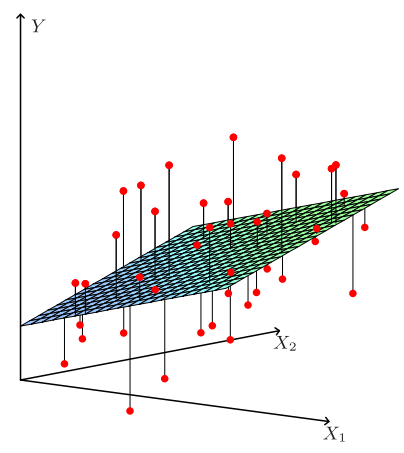
\includegraphics[width=0.3\textwidth]{images/LeastSquares.png}
	\caption{Least squares fitting. Reprinrt from \cite{ElementsStatisticalLearning}.}
	\label{fig:LeastSquares}
\end{figure}

It is common practice to centre and normalize $\mathbf{X}$ and $\mathbf{Y}$ prior to computing the $\hat \beta_{ij}$. This allow to compare the $\hat \beta_{ij}$ against each other, and makes it so that the intercept term $\beta_{0j}$ can be interpreted as the expected value of $y_{j}$. Transformation of the data can be done with $z$-scores $z_{i}=\frac{x_{i}-\bar x}{\sigma}$.

A property of the Lest Squares estimators $\hat \beta$ is that they are unbiased, and the residuals are normally distributed with zero-mean and are uncorrelated. The residual variance is defined by the sum of squares of the residuals:

\begin{equation}
\text{MLR:} \hspace{1cm} \hat \sigma^{2} = \frac{\sum^{n}_{i=1}\epsilon^{2}_{i}}{n-p-1}
\end{equation}

\begin{equation}
\text{MVLR:} \hspace{1cm} \ \hat \Sigma^{2} = \frac{\sum^{n}_{i=1}\mathbf{\epsilon_{i}}\mathbf{\epsilon_{i}}'}{n-p-1} = \frac{\sum^{n}_{i=1}(\mathbf{y_{i}}-\mathbf{\hat y_{i}})(\mathbf{y_{i}}-\mathbf{\hat y_{i}})'}{n-p-1}
\end{equation}

Additionally, the residual variance is model dependent, meaning that it depends on which predictors are used to build the linear model. Therefore, a natural question that arises is whether the particular choice of input parameters is the most adequate for the model. In general, the choice of predictors should be such to minimize residual variance. Model adequacy can be tested through several metrics. The \textit{F}-test statistic 

%\textcolor{red}{The OLS method considers only observational errors in the dependent variables, which means that  (...). The Generalized LS (GLS) method is an extension of the OLS method that considers correlations between the error terms of the regression model.  variables,  In contrast, the Total Least Squares (TLS) method takes into account observational erros in the independent variables as well.}

By replacing eq. \ref{eq:betas2} into eq. \ref{eq:OLS}, we get:

\begin{equation} \label{eq:hatMatrix}
\mathbf{\hat y}=\mathbf{X}(\mathbf{X}'\mathbf{X})^{-1}\mathbf{X}'\mathbf{y} = \mathbf{H}\mathbf{y}
\end{equation}

$\mathbf{H}$ is called the Hat-matrix, and it is useful since it maps the vector of observed values $\mathbf{y}$ onto the vector of predictions $\mathbf{\hat y}$, thus allowing to account for approximation erros when using linear regression models.

\begin{figure}[h]
	\centering
	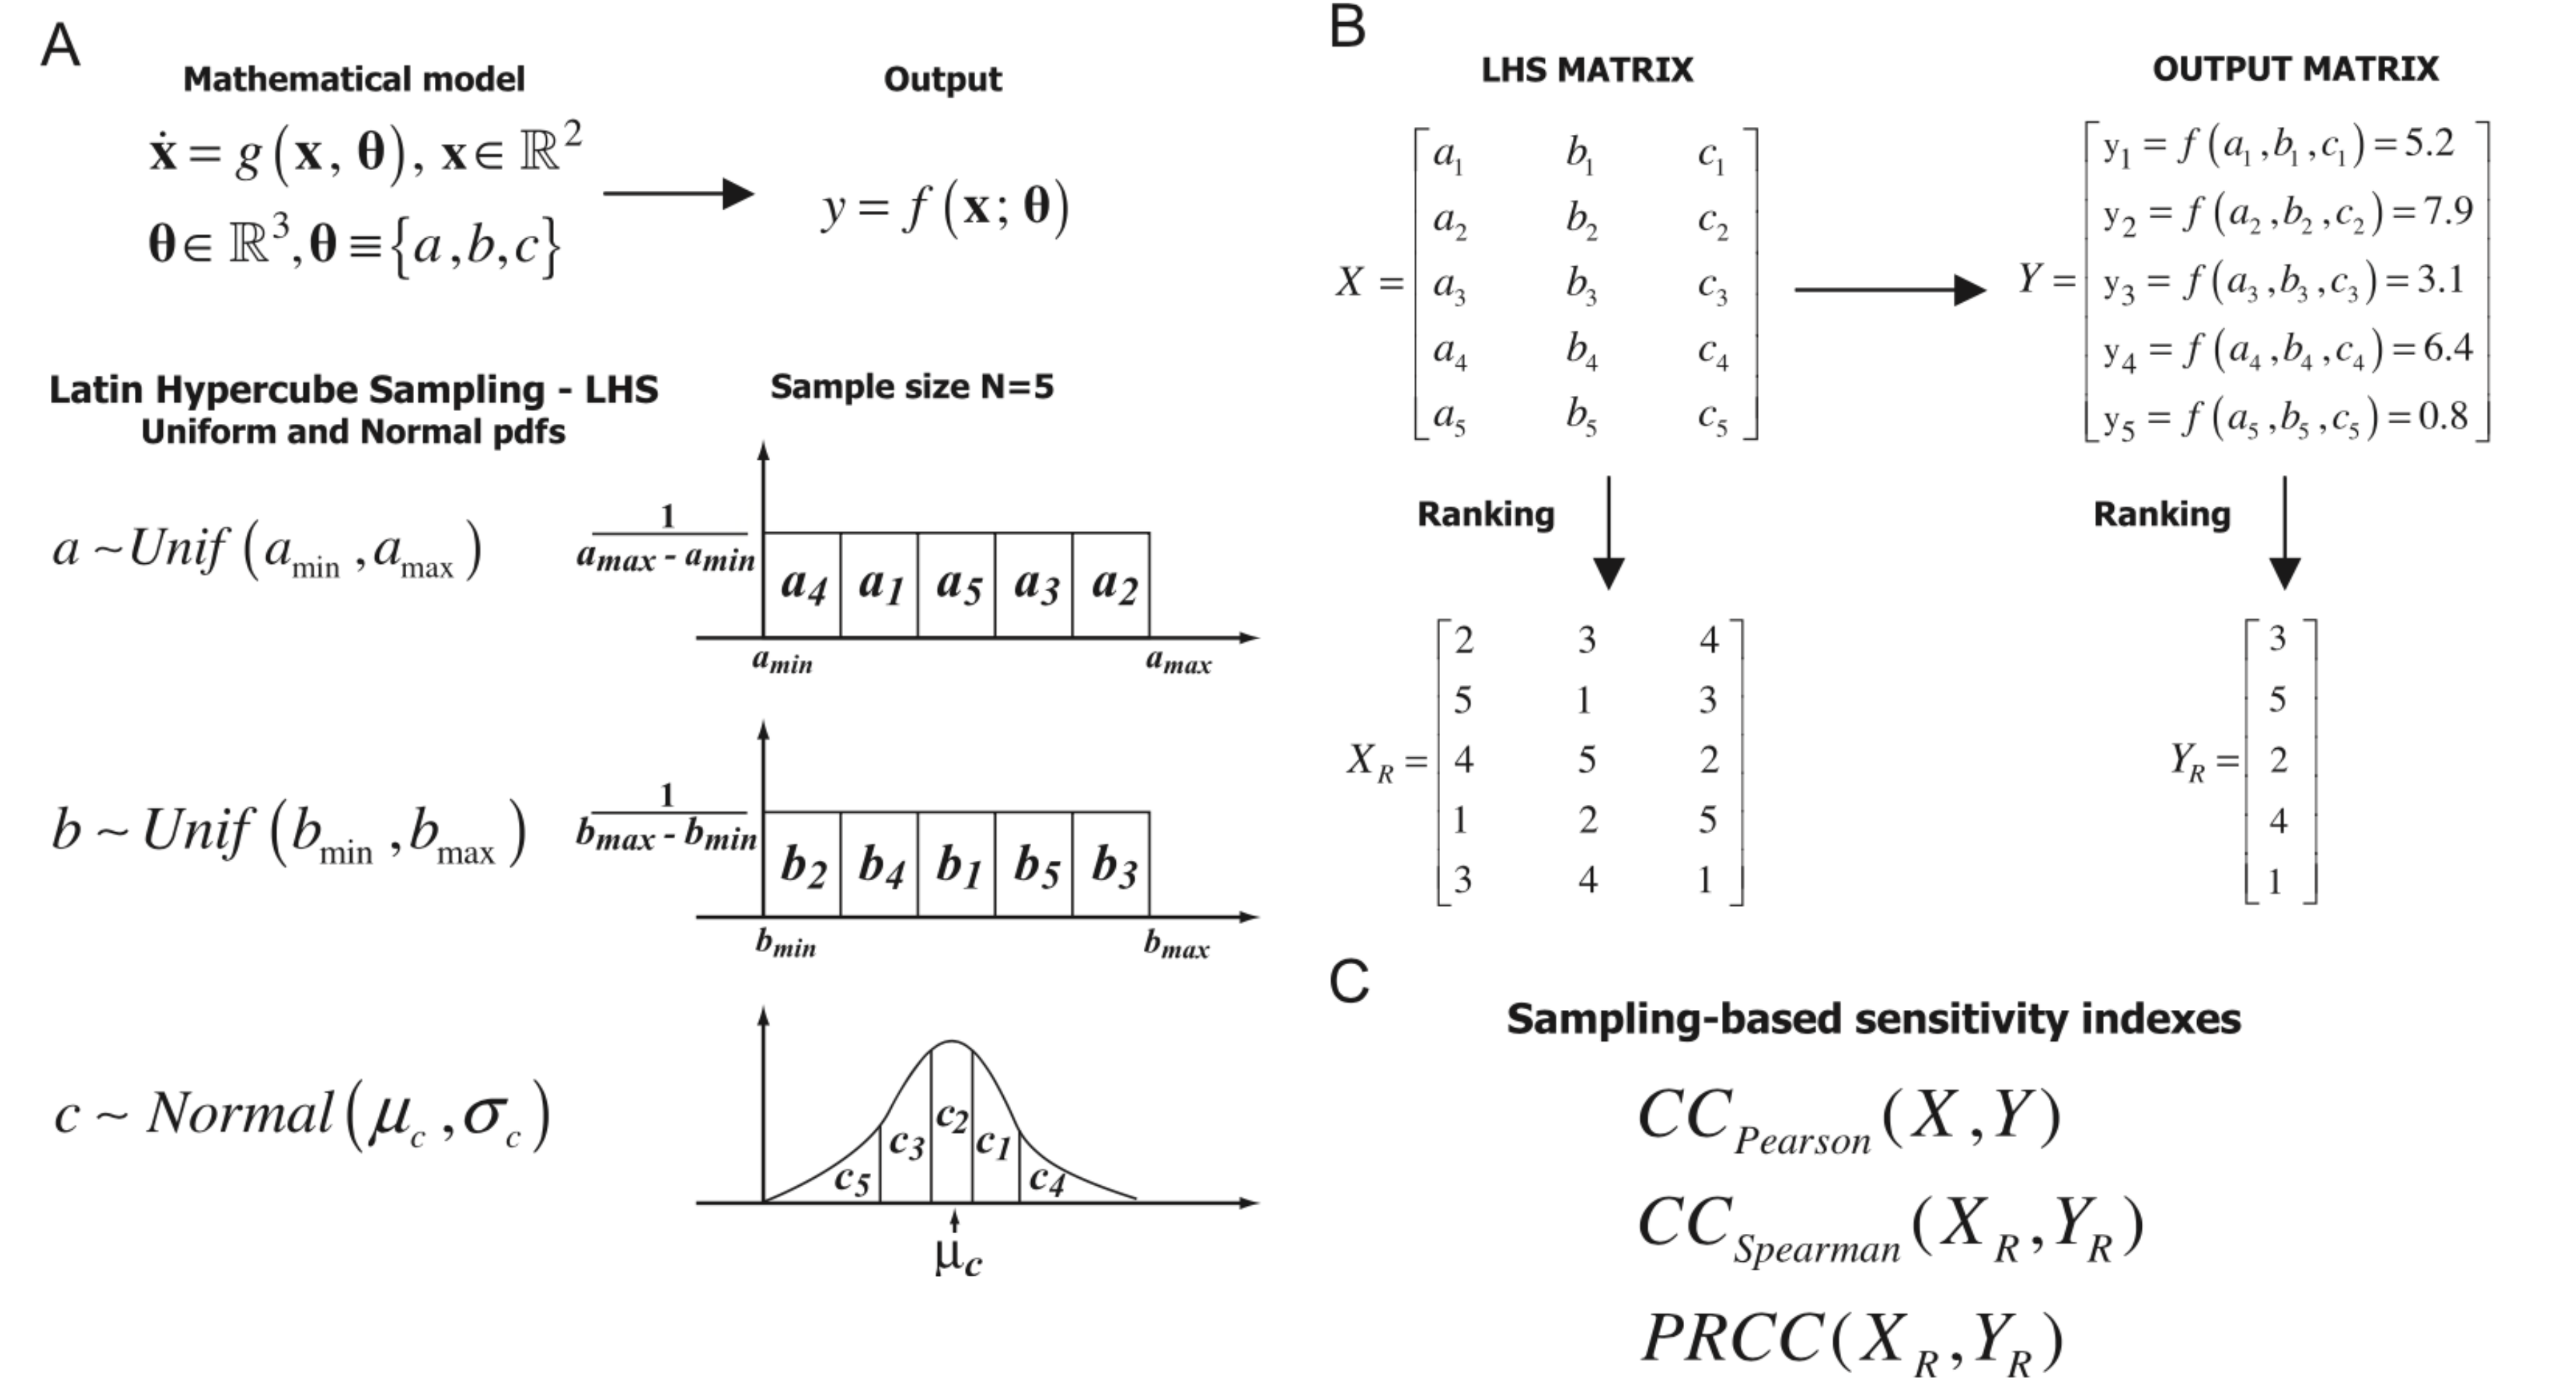
\includegraphics[width=0.8\textwidth]{images/correlation_UQ_SA2.png}
	\caption{Schematic overview of UQ and SA performed with the the LHS sampling and PRCC methods. A: the mathematical model is defined consisting of a system of ordinary differential equations. LHS method is used to randomly sample the input parameter space, where input parameter values are specified with probability distributions functions; $N_{S}=5$ samples are drawn from each distribution. B: the randomly picked samples are structured into an input matrix $X$, and $N_{S}$ simulations are run to produce the output matrix $Y$. $X$ and $Y$ are rank-transformed into $X_{R}$ and $Y_{R}$, respectively. C: Pearson correlation coefficients (CC$_{Pearson}$) are determined from $X$ and $Y$; Spearman Rank CC (CC$_{Spearman}$), and Partial Rank CC (PRCC) are determined from $X_{R}$ and $Y_{R}$. Reprint from \cite{MARINO}.}
	\label{fig:correlation_UQ_SA}
\end{figure}

%The goodness of fitness of the regression model is evaluated with the R-squared metric

\subsubsection{Model adequacy and statistical significance}

As mentioned, the sensitivity measures introduced above are based on the assumption of a linear relationship between predictive variables and model responses. The validity of the linear hypothesis can be confirmed by statistical testing.

There are several ways to evaluate model adequacy, or the ``goodness of fitness'', for regression problems. In linear regression, one common measure is the Coefficient of Determination ($R^{2}$). The $R^{2}$ represents the proportion of variation in $Y$ that is explained by the predictors, that is, how strong is the linear dependency of the variables.

This is estimated from three different sums-of-squares:
\begin{equation}
\text{Sum-of-squares Error:} \hspace{1cm} SSE=\sum^{n}_{i=1}(y_{i}-\hat y_{i})^{2}
\end{equation}
\begin{equation}
\text{Sum-of-squares Regression:} \hspace{1cm} SSR=\sum^{n}_{i=1}(\hat y_{i}-\bar y)^{2}
\end{equation}
\begin{equation}
\text{Sum-of-squares Total:} \hspace{1cm} SST=\sum^{n}_{i=1}(y_{i}-\bar y)^{2}
\end{equation}

\vspace{0.5cm}
It can be verified that $SST = SSR + SSE$. In MVLR models, these quantities become crossproducts:

\begin{equation}
\text{Sum-of-squares Error:} \hspace{1cm} SSE_{CP}=\sum^{n}_{i=1}(\mathbf{y_{i}}-\mathbf{\hat y_{i}})(\mathbf{y_{i}}-\mathbf{\hat y_{i}})'
\end{equation}
\begin{equation}
\text{Sum-of-squares Regression:} \hspace{1cm} SSR_{CP}=\sum^{n}_{i=1}(\mathbf{\hat y_{i}}-\mathbf{\bar y})(\mathbf{\hat y_{i}}-\mathbf{\bar y})'
\end{equation}
\begin{equation}
\text{Sum-of-squares Total:} \hspace{1cm} SST_{CP}=\sum^{n}_{i=1}(\mathbf{y_{i}}-\mathbf{\bar y})(\mathbf{y_{i}}-\mathbf{\bar y})'
\end{equation}

%With $SST_{CP} = SSR_{CP} + SSE_{CP                                                                                                                                           }$.


%he $R^{2}$ \textcolor{red}{is the proportion of the variance in the dependent variable that is predictable from the independent variable(s).}

%\begin{equation}
%R^{2}=1-\frac{SS_{R}}{SS_{T}}-
%\end{equation}

\begin{equation}
  R^{2}= \frac{SSR}{SST}=1-\frac{SSE}{SST}, \hspace{1cm} 0 \leq R^{2} \leq 1
\end{equation}

%\textcolor{red}{To weight the proportion of variation explained with the number of predictors, we can use the Adjusted $R^{2}$.}
%\begin{equation}
%R^{2}_{Adj}= 1-\frac{SSE/(n-p-1)}{SST/(n-1)} = 1 - \frac{\text{unexplained varianxce}}{\text{total variance}} 
%\end{equation}

%where $SST$ is the total sum of squares (proportional to the variance of the responses), and $SSR$ is the regression sum of squares (explained sum of squares).

\vspace{0.5cm}
A similar metric to the $R^{2}$ is the \textbf{\textit{F}-test} statistic. The $F$-test for regression tests the hypothesis whether any of the $p$ predictor variables have a relationship with the response, that is the ratio of explained to unexplained variance in the response:
\[
  H_{0}: \beta_{1} = \cdots = \beta_{p-1} = 0\]
\[ H_{1}: \beta_{j}  \neq 0, \text{for at least one value of j}
\]

The $F$-test compares the $F^{*}$ statistic to the \textit{F distribution}. The $F$-table \cite{Ftable} provides an estimative of the $p$-value corresponding to the $F$-value given $n$ and $p$ ($p^{*}=P(F_{p,n-p-1>F^{*}})$). 
\vspace{0.5cm}
\begin{equation}
%F = \frac{\text{explained varianxce}}{\text{unexplained variance}} 
F^{*} = \frac{SSR/p}{SSE/(n-p-1)} \sim F_{p,n-p-1}
\end{equation}

Similarly, the significance of each of the $\hat \beta$'s can be tested with a \textbf{\textit{t}-test}. The hypotheses to be tested are where a $\hat \beta_{j}$ is zero or not:

\[
H_{0}: \beta_{j} = 0, \hspace{1cm} H_{1}: \beta_{j}  \neq 0
\]

The $t$ statistic is determined as:

\begin{equation}
t = \frac{\hat \beta_{j}}{se(\hat \beta_{j})}, \hspace{1cm} se(\hat \beta_{j}) = \sqrt{\frac{SS_{E}}{(n-2)}}
%\hspace{1cm} se(\hat \beta_{j})= \frac{\sqrt{\sum^{}_{}}(y_{i}-\hat y_{j})^{2}/(n-p)}{\sum^{}_{}(x_{j}-\bar x)^{2}}%\hat \sigma(\mathbf{X}'\mathbf{X})^{-1}
\end{equation}

where $se(\hat \beta_{j})$ is the standard error of $\beta_{j}$. The $t$ statistic can be compared with the the \textit{Student's t distribution} to determined the \textit{p}-value.

A simple way to test if a group of predictors can be removed from the model, is to subdivide the predictors and respective regressors into two subgroups, with one group containing $q<p$ predictors to be tested, and the other group the remaining $p-q$ predictors. Then, a new hypothesis can be formulated:
\[
H_{0}: \beta_{q+1} = \beta_{q+2} = ... = \beta_{p} = 0
\]
\[
H_{1}: \text{at least one } \beta_{k}  \neq 0
\]

We can then build a full model and a reduced model excluding the $q$ predictors, and compare the $F^{*}$-statistic to infer on their significance.

\[
\text{Full model: } y_{i}=\hat\beta_{0}+\sum^{p}_{i=1}\hat \beta_{i}x_{ij}+\epsilon_{i} 
\]
\[
\text{Reduced model: } y_{i}=\hat \beta_{0}+\sum^{q}_{i=1}\hat \beta_{i}x_{ij}+\epsilon_{i}
\]
%\begin{equation}
%SSR(\beta_{1}|\beta_{2})=SSR(\beta_{1},\beta_{2}) - SSR(\beta_{1})
%\end{equation}

\begin{equation}
  F^{*}=\frac{(SSR_{Full}-SRR_{Red})/(p-q)}{SSE_{Full}/(n-p-1)} \sim F_{p-q,n-p-1}
\end{equation}
% A more general approach is to test whether a linear combination of the $\beta_{k}$ 
All of these statistical tests can also be performed for the MVLR problem as well.
For a more in-depth read on Linear Regression and the Least Squares method, see \cite{ElementsStatisticalLearning}.

\subsection{Correlation analysis}

Much like linear regression, correlation analysis quantifies the extent of dependence or association between two random variables, regardless of the causality relationship between them.  Correlation allows to determine  trends in the data, and therefore to make predictions of one variable given the other variable is known.
%\textcolor{red}{There are several different statistical methods allow to find correlations between input and output data by assuming certain properties of the data and an underlying regression model. CA can be performed for linear, nonlinear, monotonic and non-monotonic trends inn the data. CA encompasses a family of methods, all of them being sampling-based methods, where variable sare sampled to produce the raw data. }
For linear models, correlation is determined by the Pearson correlation coefficient (PCC):

%\begin{equation}
% \rho_{x_{i}y}=\frac{\text{Cov}(x_{j},y)}{\sqrt{\text{Var}(x_{j})\text{Var}(y)}}=\frac{\sum^{N}_{i=1}(x_{ij}-\bar x)(y_{i}-\bar y)}{\sqrt{\sum^{N}_{i=1}(x_{ij}-\bar x)\sum^{N}_{i=1}(y_{i}-\bar y)^{2}}}, j=1,2,...,k
%\end{equation}

\begin{equation}
\rho_{X_{j}Y}=\frac{\text{Cov}(X_{j},Y)}{\sqrt{\text{Var}(X_{j})\text{Var}(Y)}}=\frac{\sum^{N}_{i=1}\big(X^{(i)}_{j}-\mathbb{E}(X_{j})\big)\big(Y_{i}-\mathbb{E}(Y)\big)}{\sqrt{\displaystyle\sum^{N}_{i=1}\big(X^{(i)}_{j}-E(X_{j})\big)^{2}}\sqrt{\displaystyle\sum^{N}_{i=1}\big(Y_{i}-\mathbb{E}(Y)\big)^{2}}}
\end{equation}

%\begin{equation}
%\rho_{XY}=\frac{\text{Cov}(X,Y)}{\sigma_{X}\sigma_{Y}}=\frac{E[(X-\mu_{X})(Y-\mu_{Y})]}{\sigma_{X}\sigma_{Y}}
%\end{equation}

\[-1\leq \rho_{x_{i}y} \leq 1\]

\vspace{0.5cm}
Where $\rho_{X_{j}Y}$ is the CC between an input $X_{j}$ and the output $Y$, $N$ is the sample size, and $k$ is the number of independent variables. Cov($X_{j},Y$) is the covariance between $X_{j}$ and $Y$, and $\text{Var}(X_{j})$, $\text{Var}(Y)$ are the variances of $X_{j}$ and $Y$, respectively, and $\bar x$ and $\bar Y$ are the sample means. A $\rho_{X_{j}Y}$ close to zero indicates the absence of a linear relationship, as illustrated in Fig. \ref{fig:Correlation2}. Additionally, a negative coefficient means that the independent and dependent variables vary in opposite directions, just like in regression analysis. Note that a zero-valued $\rho_{X_{j}Y}$ does not indicate the existence of a well-defined nonlinear association between $X_{j}$ and $Y$.

\begin{figure}[h]
	\centering
	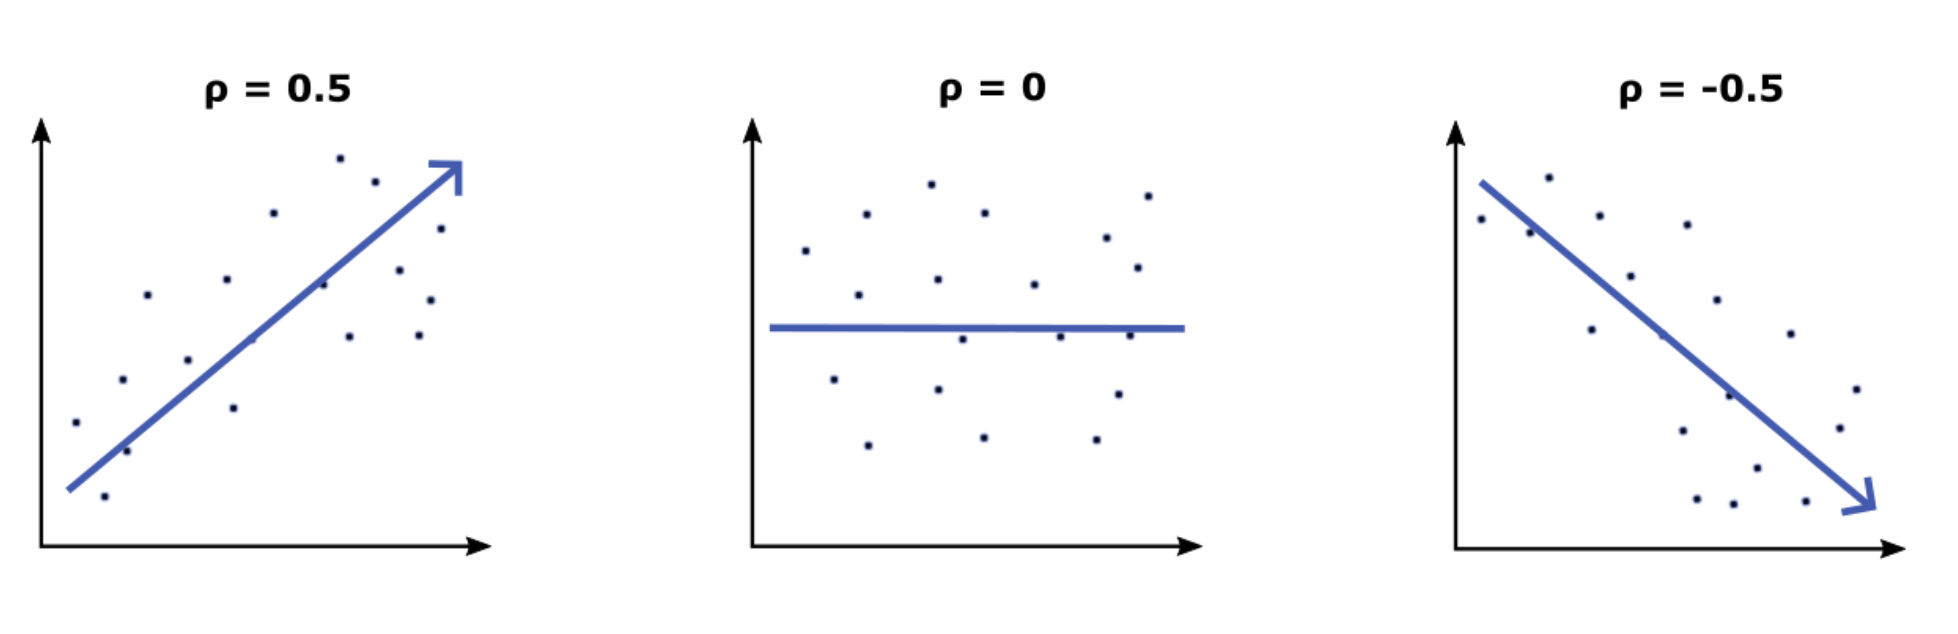
\includegraphics[width=0.7
	\textwidth]{images/correlation3.png}
	\caption{Schematic representation of correlation coefficients for three different types of data.}
	\label{fig:correlation2}
\end{figure}

As previously mentioned, the Pearson correlation coefficient provides a measure of strength of linear association between $X_{j}$ and $Y$, and therefore can be used as sensitivity indices to rank variable importance. Unlike regression coefficients, which are influenced by the distributions assigned to $X_{j}$, correlation tends to exclude the effects of other independent variables, as well as their assumed distributions.  If two random variables are statistically independent, the value assigned to one variable does not affect the probability distribution of the other. However, if correlations between the independent variables exist, this is no longer the case, and analyses based on the Pearson CC can be inaccurate. Note that, if $X_{j}$ are all statistically independent, the PCCs and SRCs give the same variable importance rankings. Like in regression analysis, CC are more of a qualitative SA than quantitative.

\vspace{0.5cm}
To improve the accuracy of the PCC when one variable is numerically associated with $X_{i}$, partial correlation coefficients can be used instead.  \textbf{Partial correlation} characterizes the linear relationship between  $X_{j}$ and  $Y$ after the linear effects of the remaining inputs are discounted. This is done by building two regression models: 

\begin{equation}
	\widehat{X_{-j}}= c_{0}+\sum^{n}_{\substack{p=1\\p\neq j}} c_{p}X_{p}
\end{equation}

\begin{equation}
\widehat{Y_{-j}}= b_{0}+\sum^{n}_{\substack{p=1\\p\neq j}} b_{p}X_{p}
\end{equation}

	%$\hat x_{j}$ and $\hat y$ are obtained from the MLR regression model presented in section }\ref{sec:MLR}.
where $\widehat{X_{-j}}$ denotes the prediction of the linear model expressing $X_{j}$ in relation to the other inputs, and  $\widehat{Y_{-j}}$ is the prediction of the linear model without $X_{j}$. Thus, two new variables can be defined as $(X_{j}-\widehat{X_{-j}})$, and $(Y-\widehat{Y_{-j}})$, with the partial correlation coefficients being the CC between the residuals $(X_{j}-\widehat{X_{-j}})$ and $(Y-\widehat{Y_{-j}})$:

\begin{equation}
\hat \rho_{X_{j}Y}=\rho(X_{j}-\widehat{X_{-j}},Y-\widehat{Y_{-j}})=\frac{\text{Cov}\big(X_{j}-\widehat{X_{-j}},Y-\widehat{Y_{-j}}\big)}{\sqrt{\text{Var}\big(X_{j}-\widehat{X_{-j}}\big)\text{Var}\big(Y-\widehat{Y_{-j}}\big)}}
 %=\frac{\sum^{N}_{i=1}(x_{ij}-\hat x_{j}-\bar x)(y_{i}-\hat y-\bar y)}{\sqrt{\sum^{N}_{i=1}(x_{ij}-\hat x_{j}-\bar x)\sum^{N}_{i=1}(y_{i}-\hat y-\bar y)^{2}}}, j=1,2,...,k
\end{equation}


\vspace{1cm}
The \textbf{\textit{T}-test} statistic allows to test the significance of a CC (if it significantly differs from zero), and if two CCs are significantly different from each other:

\begin{equation}
T=r \sqrt{\frac{(N-2-p)}{1-r^{2}}} \sim t_{N-2-p}
\end{equation}

\vspace{0.5cm}
where \textit{T}  follows a Student's \textit{t} distribution with $(N-2-p)$ degrees of freedom, and $p=0$ for the Pearson CCs. Again, $N$ is the sample size, and $p$ is the number of inputs whose effects are discounted when calculating the CCs. The significance can be inferred from the corresponding $p$-value of the $t$ distribution. 

In order to test if two CCs ($r_{1}, r_{2}$) are significantly different from each other, the \textbf{$Z$-test} can be performed on log transformed CCs:

\begin{equation}
  \dot r=\frac{1}{2}ln\mid\frac{1+r}{1-r}\mid: N(\mu,\frac{1}{\sqrt{N-3-p}})
\end{equation}

\vspace{0.5cm}
where again $p$ is the number of inputs whose effects are discounted when calculating the PRCCs, and $p=0$ for the Pearson CCs. The log-transformation is used here to conform the data to the normal distribution. The significance can be inferred from the corresponding $p$-value of the normal distribution. 

\begin{equation}
  z=\frac{\dot r_{1}-\dot r_{2}}{\sqrt{\frac{1}{N_{1}-3-p_{1}}+\frac{1}{N_{2}-3-p_{2}}}}: N(0,1)
\end{equation}

\vspace{0.5cm}

\subsubsection{Non-linearities in the model}

The above mentioned statistical test allow to test the validity of the linearity hypothesis. If the linearity between inputs and outputs cannot be assumed, the above mentioned sensitivity measures can still be used by applying a \textbf{rank transformation} to the data, providing that outputs vary monotonically with the inputs. 
The data $(X^{n},Y^{n})$ is rank transformed to $(R^{n}_{X},R^{n}_{Y})$ by replacing the values in each column by their respective ranks. 

The equivalent of the Standard Regression Coefficient for rank transformed data is the Standard Rank Regression Coefficient (SRCC). Similarly, the Pearson CC becomes the Spearman Correlation Coefficients, or the Spearman Rho, and the PCC becomes the Partial Rank Correlation Coefficients (PRCC).  PRCC is a robust sensitivity measure for non-linear but monotonic relationships between $X_{j}$ and $Y$ as long as little or no correlation exists between the inputs. Figure \ref{fig:Correlation} shows an example of the different types of CCs of the same variables, showing that these can uncover substantially different trends in the data. 

Other methods that can be used for nonlinear models are nonlinear regression, where the $X_{i}$ variables are expressed as functions of nonlinear operators, such as exponentials and sinusoids.  Another commonly used technique is nonparametric regression. These methods will not be covered in the present essay, but more detailed information can be found in \cite{HELTON20061175,SaltelliThePrimer}

Graphical techniques can also be quite useful in SA for detecting nonlinear or other major relationships between the inputs and outputs. Therefore, inspection of scatterplots constitutes a natural starting point in the analysis of complex systems, and can provide insight into the most appropriate SA strategy. For instance, scatter plots allow to visually inspect the nature of the trends in the data, as exemplified in Fig. \ref{fig:Correlation}. Although scatter plots allow to infer the nature of the dependencies in the model, it does not provide information on the interaction effects among input variables. Therefore, it usually requires some level of knowledge of the most significant interactions in order to select the variables to display on the same 2D or 3D plot. Other types of plots, such as coweb plots \cite{UncertaintyAnalysis}, can help visualize common trends in the data by plot ``simulation trajectories'' of the input parameters, as show in Fig. \ref{fig:Coweb_plot}.   

%Note that the regression analysis presented in section \ref{sec:MLR} can also be performed in exactly the same way with rank-transformed data, thus yielding Standardized Rank Regression Coefficients (SRCC). 

\begin{figure}[h]
	\centering
	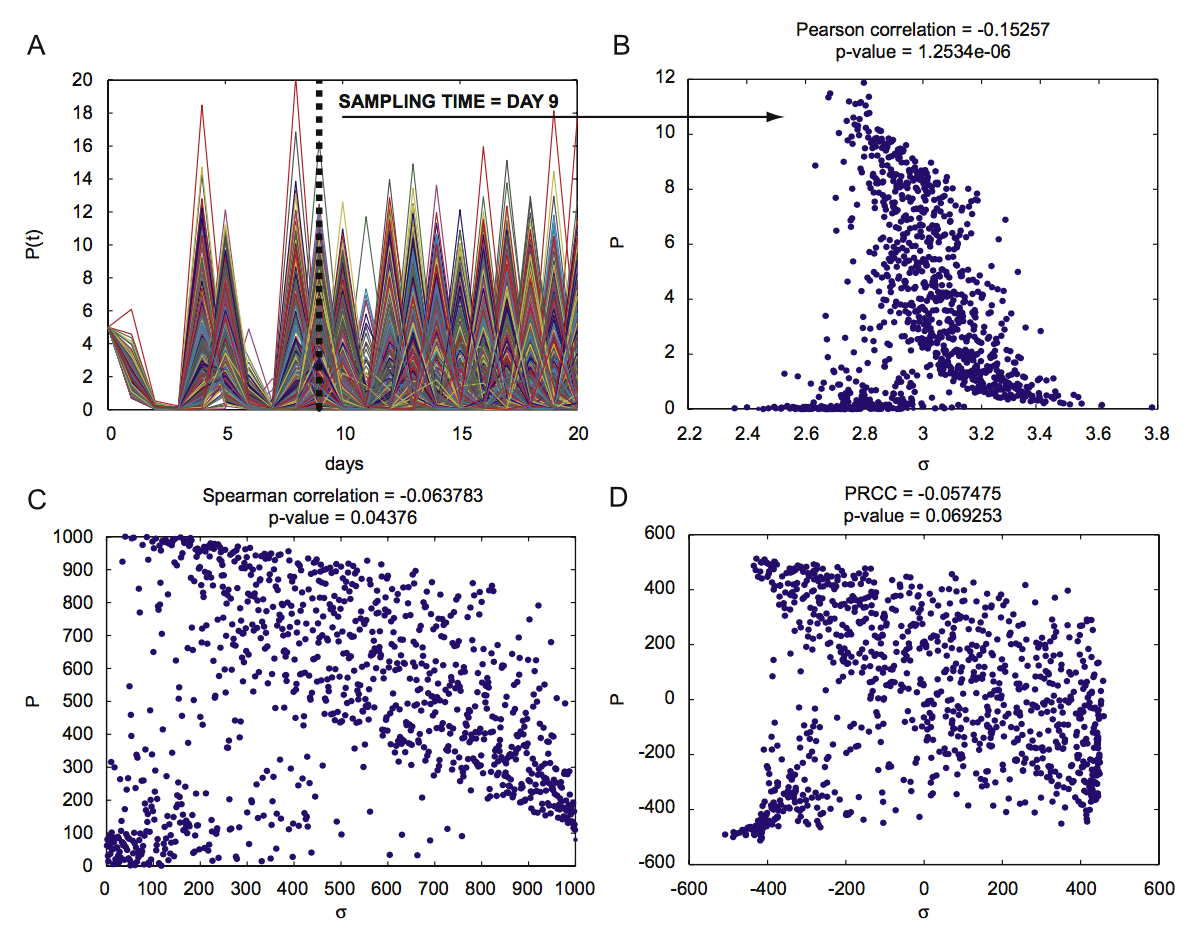
\includegraphics[width=0.65\textwidth]{images/Correlation2.png}
	\caption{Plot of the output of the Lotka-Volterra model (A), in respect to one of its input variables, and scatter plots showing the Pearson CC (B), the Spearman CC (C), and the PRCC. Reprint from \cite{MARINO}.}
	\label{fig:Correlation}
\end{figure}

\begin{figure}[h]
	\centering
	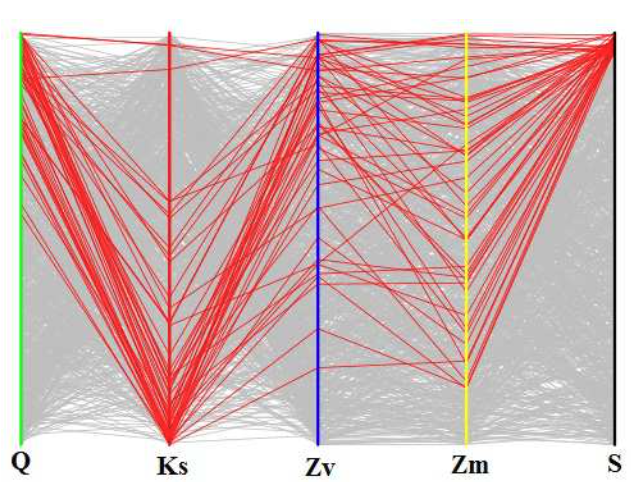
\includegraphics[width=0.45\textwidth]{images/Coweb_plot.png}
	\caption{Example of a coweb plot showing a set of trajectories of the simulations corresponding to the 5\% largest output values. Reprinted from \cite{iooss:hal-00975701}.}
	\label{fig:Coweb_plot}
\end{figure}

\FloatBarrier

\subsection{Sobol indices}
\label{sec:Sobol}

When models are non-linear and non-monotonic, the preferred choice pf SA method is the so-called \textbf{variance-based SA}. This method is based on \textit{functional decomposition of variance}, whereby variance in the model output is decomposed into fractions of variance attributable to inputs of groups of inputs. This method (as well as the eFAST method presented in the next section) is closely related to analysis of variance (ANOVA), and so it falls into the general framework of \textbf{ANOVA-like decomposition} of factorial analysis \cite{ANOVA}. Importantly, in contrast to regression and correlation analysis, variance decomposition methods can provide actual quantitative measures of sensitivity, and they are model independent in the sense they they do not require the model to be linear or monotonic to be effective. 

There are several ways in which to variance can be decomposed, but once the variance fractions are known, it is possible to estimate sensitivity indices as ratios of the fractional variance of inputs to the total variance in the output. This framework was  introduced by \'{I}lia Sobol, and thus the sensitivity indices are known as Sobol Indices \cite{SOBOL1993,SOBOL2001}. 

%The Sobol Decomposition method was first introduced by \cite{SOBOL1993} \textcolor{red}{as a generalization of the method developed by \cite{CUKIER19781}, and then presented more consistently in \cite{SOBOL2001}}. 

Consider the mathematical model described by the function $Y=f(\mathbf{X})$, where $\mathbf{X}=(X_{1}, ..., X_{n}) $ is a vector of input parameters defined in a unit $n$-dimensional unit cube denoted by $I^{n}$, such that each $0\leq X_{i}\leq 1$. If $f(\mathbf{X})$ is integrable and defined in $I_{n}$, $f(\mathbf{X})$ can be decomposed in an expansion of  orthogonal summands of different dimensions (i.e., dependencies on input parameters of different orders):

%\begin{equation}
  %   f=f_{0}+\sum^{n}_{s=1}\sum^{n}_{i_{1}<...<i_{s}}f_{i_{1}...i_{s}}(x_{i_{1}},..., x_{i_{s}}), 1\leq i_{i}<...<i_{s}\leq n
%\end{equation}

\begin{equation}
f=f_{0}+\sum^{}_{i}f_{i}(X_{i})+\sum^{}_{i<j}f_{ij}(X_{i}, X_{j})+\cdots+f_{12\cdots n}(X_{1},\cdots, X_{n}), 
\end{equation}

With total number of summands equal to $2^{n}$, $f_{0}$ is constant and integrals of the $f_{i_{1}\cdots i_{s}}$ are all zero (orthogonality). This expansion is unique if:

\begin{equation}
	\int_{0}^{1}f_{i_{1}\cdots i_{s}}(x_{i_{1}},\cdots,x_{i_{s}})dx_{i_{k}}=0,1\leq k\leq s, \{i_{1},\cdots,i_{s}\}\in\{1,\cdots,n\}
\end{equation}
\[1\leq i_{i}<...<i_{s}\leq n\].

%More recently, this expansion has also been referred to as ANOVA-representation of $f(x)$, or \textit{surrogate} model.
 It follows that $f_{0}$ is a constant:
\begin{equation}
\int^{}_{}f(\mathbf{X})d\mathbf{X}=f_{0}.
\end{equation}

where $f_{0}=\mathbb{E}[Y]$ is a constant representing the expectation, or mean value, of the output.  By assuming that all integrals of $f(\mathbf{X})$ are square integrable in $I^{n}$, we can find the relationship:
\begin{equation}
	\int^{}_{}f^{2}dX-f^{2}_{0}=\sum^{n}_{s=1}\sum^{n}_{i_{1}<\cdots<i_{s}}\int^{}_{}f^{2}_{i_{1}\cdots i_{s}}dx_{i_{1}}\cdots dx_{i_{s}}.
\end{equation}

\vspace{0.5cm}
The above relationship can be represented in terms of the variances:
\begin{equation} \label{eq:Variances}
\begin{split}
\text{Var}(Y) & =\sum^{n}_{s=1}\sum^{n}_{i_{1}<\cdots<i_{s}}D_{i_{1}\cdots i_{s}}(Y)= \\
& = \sum_{i=1}^{n} D_{i}(Y) + \displaystyle\sum_{i<j}^{d} D_{ij}(Y) + \dots + D_{1,\dots,n}(Y)
\end{split}
\end{equation}
where $\text{Var}(Y)$ denotes the variance of $Y$, the term $D_{i}(Y)$ denotes the variance associated with variable $X_{i}$, and $D_{ij}(Y)$ denotes the variance associated with the interaction between variables $X_{i}$ and $X_{j}$. The relationship above represents the partitioning of the total variance in the output ($D(Y)$) into components of increasing dimensionality ($D_{i_{1}\cdots i_{s}}$). The terms on the first summation on the right-hand side of equation \ref{eq:Variances} represent the contribution from each $X_{i}$ to the variance of $Y$; the second summation represents the variance attributed to the interaction between different variables. 
%The output variance $V_{i}$ is defined as the output variance when  $x_{i}$ assumes a given value, given all other variables of the model. 

The Sobol method decomposes the variance observed in the model output $\mathbf{Y}$ into the contributions associated to each of the input variables ${X_{i}}$, that is, their 'importance' to the variance in the output $Y$. %Thus, this method falls into the category of \textbf{variance-based methods}, which includes the ANOVA-like decomposition methods.
The single impact of $x_{i}$ is given by the conditional variance of $Y$ ($D(Y)$) by fixing only $X_{i}$ to a single value:

\begin{equation}
D_{i}(Y)=\text{Var}[\mathbb{E}(Y|X_{i})]
\end{equation}

%where $u$ represents a particular point estimate of $x_{i}$ , and $x_{-i}$ denotes the set of all variables except $x_{i}$.  Since $u$ is unknown,  each instance of $x_{i}$ results in a different conditional variance, given that all other variables are fixed. 
%The smaller the conditional expectation of the variable $Y$, given that $x_{i}=X^{*}_{i}$, $E_{x_{i}}(V_{x_{}i})(y|X_{i})$, the more important the variance of $X_{i}$ for the variance of $Y$. 

One of the strengths of the Sobol method method is that it allows to take into consideration the variance associated with an input. The impact of the interaction between variables $x_{i}$ and $x_{j}$ is given by:
\begin{equation}
D_{ij}(Y)=\text{Var}[\mathbb{E}(Y|X_{i},X_{j})]-D_{l}(Y)-D_{j}(Y)
\end{equation}

The variance of the distribution of the outputs can then be used to calculate sensitivity indices of $Y$ to the inputs. These are called Sobol indices (SI). The SI are naturally derived by normalizing the decomposition of variances presented above to the variance in the output:

\begin{equation}
	S_{i}=\frac{D_{i}(Y)}{D(Y)} , \hspace{1cm} S_{i_{1}\cdots i_{s}}=\frac{D_{i_{1}\cdots i_{s}}(Y)}{D(Y)} 
\end{equation}

These ratios are  global sensitivity indices since they capture the variance attributed to the variables directly and via interaction with other variables. All $S_{i_{1}\cdots i_{s}}$ lie in the range $[0:1]$ and their sum is equal to 1:

\begin{equation}
	\sum^{n}_{s=1}\sum^{n}_{i_{1}<\cdots<i_{s}}S_{i_{1}\cdots i_{s}}=\sum^{n}_{i}S_{i}+\sum^{n}_{i<j}S_{i\cdots j}=1
\end{equation}

\vspace{0.5cm}
The Sobol indices $S_{i}$  are called ``first-order sensitivity indices'', or ``main effect indices''. They quantify how much the total variance of the model is reduced by \textit{fixing} the $i$th parameter. Indices $S_{i...j}$ represent the higher order SI, quantifying the mixed effects of fixing $x_{i}$ in the variance of the other variables; these can be used to assess the degree of interdependency of the variables.

The total-order sensitivity indices $S^{T}_{i}$ correspond to the total part of the output variance attributed to each $X_{i}$, including the marginal effect and the interactions effects with other parameters: 
%\begin{equation}
%S^{T}_{i}=\frac{\mathbb{E}_{X_{-i}}(D(Y|X_{-i}))}{D(Y)}=1-\frac{D_{X_{-i}}(\mathbb{E}_{X_{i}}(Y|X_{-i}))}{D(Y)}
%\end{equation}

\begin{equation}
S^{T}_{i}=S_{i}+\sum^{}_{i<j}+\sum_{j\neq i,k\neq i,j<k}S_{ijk}+\cdots =\sum_{l\in {\#}i}S_{i}
\end{equation}

\vspace{0.5cm} 
where $\#i$ are all subsets of $\{1,...,d\}$ that include $i$. For instance, in a model with 3 independent variables, the total SI of the parameters 1 would be $S^{T}_{1}=S_{1}+S_{12}+S_{13}+S_{123}$.  $S^{T}_{i}$ also takes into account the variance attributable to interactions with other variables.  The larger the $S_{i}$ and the $S^{T}_{i}$, the more sensitive the model is to that variable. SI are analogous to the $R^{2}$ in regression, which represent the proportion of variance explained by parameter $x_{i}$. 

The total-order indices encode the contributions of parameters through non-linear of interaction effects. If these interaction effects are negligible (all parameters are uncorrelated), then

\begin{equation} \label{eq:totaleffects}
	\sum^{n}_{i=1}S_{i} \simeq 1.
\end{equation}

In this case, the model is said to be \textit{additive}. If the sum in eq. \ref{eq:totaleffects} is $>1$, then the interaction effects have to be considered. 

There are several advantages of using variance-based methods for GSA:
\begin{itemize}
	\item They allow to compute the sensitivities of the model across the whole input space;
	\item They can deal with non-linearities in the model; 
	\item They take into account the interactions between input variables in non-additive systems.
\end{itemize}



\vspace{0.5cm}
%\subsubsection{Computation of the Sobol indices}

In order to compute the Sobol indices of a process, each component of the variance has to be computed. The The Sobol Indices can be computed with Monte Carlo sampling \cite{SOBOL1993,SALTELLI2002280}, but this method can be very computational costly for complex and non-linear models. Therefore, other schemes such as quasi-Monte Carlo, and FAST \cite{CUKIER19781,SaltelliFAST} have been used to reduce the computational cost.  
With MC, the Sobol Indices can be directly computed from $f(x)$ by estimating the expected values of the quantities from multiple model evaluations.
The Sobol Indices can also be directly estimated from a surrogate model $f^{\prime}$, with analytical solution of the integral components. For instance, the variance decomposition of the Polynomial Chaos Expansion presented above have an exact form, and therefore the SI can be computed analytically.
%It is also noticeable the similarity between the Sobol Decomposition and the PCE presented earlier. Both methods decompose a given model funciton into $p$ orthogonal terms with a defined pdf. \textcolor{red}{The PCE is a particular case of the Sobol decomposition, where the summands of the expansion are all represented by polynomial functions}. in the case of a PCE, the model is replaced by a surrogate model obtained with the PCE, and the Sobol sensitivity indices can then be computed from the variance terms of the expansion:

%\begin{equation}
%	D_{i}=\int^{}_{}\hat f_{i}^{2}(x)dx=\int^{}_{}\left(\sum^{}_{n}C_{n}\Phi_{n}(x)\right)^{2}dx
%\end{equation}

\subsection{Fourier Amplitude Sensitivity Test}

An alternative method to determine sensitivity indices based on decomposition of variance was proposed  by Cukier et al.: the Fourier Amplitude Sensitivity Test (FAST) \cite{Cukier1973,CUKIER19781}. This method was originally developed in the context of the analysis of coupled chemical reaction systems for the computation of the first order sensitivity indices. Later, Satelli et al. \cite{SaltelliFAST} developed the extended FAST (eFAST) method based on the original FAST algorithm which allowed also to calculate total-order sensitivity indices. 
Similar to the Sobol method, FAST partitions the variance in the output  among the contributions of each input variable. The key difference is that the FAST method uses a sampling scheme based on sinusoidal functions, and multiple Fourier series decomposition for the partitioning of the variance. One main advantage of the FAST and eFAST method over other variance-based methods is its lower computational cost due to the efficient sampling scheme it uses. 

Consider again the model $Y=f(\mathbf{X})$, with $\mathbf{X}=\{X_{1},X_{2},\cdots,X_{k}\}$. The method works by varying each model parameter at a different set of integer frequencies, which serves as a unique identifier of that parameter.
In the first step, each input parameter is transformed into a new independent variable $s$, and sampled with a one-dimensional sinusoidal function called \textit{search curve}. The search curve explores the entire $n$-dimensional input space with multiple parameter combinations.  

\begin{equation}
x_{l}(s)=G_{l}(\sin w_{l}s), \forall l=1,2,\cdots,n, -\infty<s<+\infty
\end{equation}

where $s$ is a scalar parameter, $G_{i}$ is a transformation function, and $\{w_{i}\}$ are a set of different frequencies associated to each input factor. $f(\mathbf{X})$ can then be expressed as $f(s)=f(X_{1}(s),...,X_{n}(s))$.  The exact form of $x_{i}(s)$ depends on the sampling distribution desired. Saltelli et al. \cite{SaltelliFAST} proposed the following as transformation function, although other functions have also been proposed \cite{Cukier1973,CUKIER19781}:

\begin{equation}
x_{l}(s)=\frac{1}{2}+\frac{1}{\pi} \arcsin(\sin(w_{l}s+\phi_{l})), \forall l \in [1,n]
\end{equation}

%\begin{equation}
%  x=f(N_{s})
%\end{equation}
\vspace{0.5cm}
where $N_{s}$ is the number of samples per parameter, and it is equal to $2Mw_{max}+1$, where $M$ is an interference factor (typically 4), and $w_{max}$ is the maximum frequency assigned to the parameter. The original model $f(\mathbf{x})$ is therefore expressed as a function of a single independent variable: $y=f(s)=f(x_{1}(s),x_{2}(s),\cdots,x_{N}(s))$.

A set of rules dictate which values of frequencies are allowed such that the search curve forms a closed path covering the entire input space. According to the Nyquist-Shannon sampling theorem, the frequencies must less than 1/2 of the sampling frequency to avoid aliasing effects. Additionally, to ensure that the whole parameter space is explored, the set of frequencies $w_{l}$ chosen for each $x_{i}$ must not be a linear combination %($\sum^{n}_{i=1}\gamma_{i}w_{i}\neq 0$) 
of the remaining frequencies, i.e., have no harmonics in common (incommensurate). 
If this is the case, the search curve covers the entire input space as $s$ varies from 0 to $+\infty$, and according to the ergodic theorem, it is possible to express the variance of $f(\mathbf{X})$ (which is a multi-dimensional integral of $(X_{1},X_{2},...,X_{N})$) as a one-dimensional integral of $s$:

\begin{equation}
\sigma^{2} = \frac{1}{2\pi}\int^{\pi}_{-\pi}f^{2}(s)ds - \Bigg[\frac{1}{2\pi}\int^{\pi}_{-\pi}f(s)ds\Bigg]^{2}.
\end{equation}

\vspace{0.5cm}

%The frequencies assigned to each parameter must meet certain criteria to ensure that the parameters do not take irrational values.  
Additionally, if $w_{i}$ are positive integers, then $f(s)$ is periodic in $(-\pi;\pi)$ \cite{Cukier1973}.
% From this, the total variance $\hat D$ can be calculated as:
The frequencies encoded in each parameter is then propagated through the model by performing several model evaluations with the parametric search curves. The frequencies can then be detected in the output by computing the Fourier coefficients of the model results. The Fourier coefficients can be computed as one-dimensional integrals, assuming the fundamental frequencies follow the properties explained above. The Fourier series of $f(s)$ and its coefficients are defined as:
\begin{equation}
f(s)=\sum^{+\infty}_{p=-\infty}\{A_{pw_{l}}\cos (pw_{l}s) + B_{pw_{l}}\cos (pw_{l}s)\}
\end{equation}
\begin{equation}
A_{pw_{i}}=\frac{1}{2\pi}\int^{\pi}_{-\pi}f(s)\cos(pw_{l}s)ds%, \hspace{0.5cm} p=0,1,...
\end{equation}
\begin{equation}
B_{pw_{i}}=\frac{1}{2\pi}\int^{\pi}_{-\pi}f(s)\sin(pw_{l}s)ds%, \hspace{0.5cm} p=1,2,...
\end{equation}
\[p \in \mathbb{Z}=\{-\infty, \cdots,-1,0,1,\cdots,\infty\}, \]
where $A_{pw_{l}}$ and $B_{pw_{l}}$ are the real and imaginary parts of the Fourier coefficients of the $l$th parameter. Note the infinite integral in the equation above as a consequence of the transformed function $f(s)$ being periodic in $2\pi$. To evaluate the above integrals, the input space is sampled by drawing $N$ values from $s_{k}=\frac{2k\pi}{N}, k=1,...,N$.

According to Parseval's Theorem, the marginal and total variances, $\sigma^{2}_{i}$ and $\sigma^{2}$, can then be estimated from the Fourier coefficients for each fundamental $w_{l}$ and its harmonics, $pw_{l}$, as:

\begin{equation} 
%D_{i}=\int^{1}_{0}f^{2}_{j}(X_{j})dX_{j}=2(A^{2}_{j}+B^{2}_{j})
\sigma^{2}_{l}=2\sum^{+\infty}_{p=-\infty}(A^{2}_{pw_{l}}+B^{2}_{pw_{l}})
\end{equation}

\begin{equation}
\sigma^{2}=2\sum^{+\infty}_{j=-\infty}(A^{2}_{j}+B^{2}_{j})
\end{equation}

\vspace{0.5cm}
where $p\neq 0$ and $j\neq 0$, and $(A^{2}_{j}+B^{2}_{j})$ are the sum of of squares of the Fourier coefficients of all integer frequencies (total variance). In practice, integer frequencies are only approximately incommensurate to an order of $M$, and thus $A_{pwi}, B_{pwi}$ can only be approximated with a given error, $A^{*}_{pwi}, B^{*}_{pwi}$.

The partial variance of parameter $X_{l}$ (the fraction of variance of the output due to the uncertainty in the $l$th parameter when the output is averaged over the uncertainties of all the other parameters $X_{i}, i\neq l$) is given by:
\begin{equation}
S^{*}_{w_{l}}=\frac{\sum^{N/2}_{p=-(N/2-1)}(A^{*}_{pw_{l}}|^{2}+B^{*}_{pw_{l}}|^{2})}{\sum^{N/2}_{j=-(N/2-1)}(A^{*}_{j}|^{2}+B^{*}_{j}|^{2})}=\frac{(\sigma^{*}_{i})^{2}}{(\sigma^{*})^{2}}
\end{equation}

 This is the main effects of the parameter $X_{l}$. The parameters with the largest influence on the output correspond to the highest frequency components in the frequency spectrum. 

\vspace{0.5cm}
The \textbf{eFAST} method \cite{SaltelliFAST} was introduced as a variation of the well-established FAST to allow for the calculation of total-order effects o any input variable. In eFAST, each $X_{i}$ is varied at a high frequency, while varying the remaining parameters at low and non-unique frequencies. This provides an estimate of the contributions of the complementary set of $i$ (that is, the variance attributable to all all parameters expect $i$, thus allowing to calculate the total-order sensitivity indices, $S^{T}_{i}$. The remainder portion of variance that that is not accounted for by the first-order or total-order indices corresponds to non-linear or interaction effects. This,  $S^{T}_{i}$  can also be used to infer the degree of additivity of the model.

The error made in the estimations of the variance components can be reduced by performing $N_{R}$ resampling with different parameter search curves, each specified by a random phase shift,  and then by taking the mean of the calculated variances. the eFAST algorithm is then repeated $k\times N_{S}\times N_{R}$ times to perform a full SA.

Marino et al. \cite{MARINO} proposed a method for determining the statistical significance of the sensitivity indices obtained with the eFAST method. They proposed to include of a dummy parameter in the analysis (in this case, a parameter non-existent in the model), which will result in a non-zero sensitivity index due to aliasing or interaction effects. Since in the eFAST method the input space is randomly sampled $N_{R}$ times, it yields multiple estimates of the variance associated with each parameter. Then, a two-sample $t$-test can be used to compare the distributions of the estimated sensitivity measures $S_{i}$ and $S^{T}_{i}$ of each input parameter with those of the dummy parameter. The null hypothesis is that parameters with total-order sensitivity index less than or equal to that of the dummy parameter should not be considered significant. For further details see supplementary material of \cite{MARINO}.

%The total sensitivity indices proposed by Saltelli et al. \cite{SaltelliFAST}, are calculated based on 

%Assuming the model to be a function $Y=f(X)$, with $X={X_{1}, X_{2}, ..., X_{p}}$, and assuming that all inputs are independently and uniformly distributed, and $X_{i} \in [0, 1]$ for $i=1,2,...,p$, $f(X)$ can be decomposed as:

%\begin{equation}
%Y=f(X)=f_{0}+\sum^{n}_{j=1}f_{j}(X_{j})+\sum^{p}_{i<j}f_{ij}(X_{i},X_{j})+ \cdots +f_{1,2,...,n}(X_{1}, X_{2}, ..., X_{d})
%\end{equation}

%\begin{equation}
%\text{Output variance:} \hspace{1cm} \sigma^{2}=\frac{\sum^{N}_{i=1}(y_{i}-\bar y)^{2}}{N-1}
%\end{equation}

%\begin{equation}
 % Y=f(X)=f_{0}+\sum^{n}_{j=1}f_{j}(X_{j})+\sum^{n-1}_{j=1}\sum^{n}_{k=j+1}f_{jk}(X_{j},X_{k})+ \cdots +f_{12...n}, j=1,2,...,n
%\end{equation}
%where $0\leq X_{j}\leq 1$.

\vspace{0.5cm}
To illustrate how this method works, Fig. \ref{fig:FAST} shows the results of performing eFAST on the Lotka-Volterra of predator-prey dynamics from \cite{MARINO}. Input parameters $\sigma$ and $\beta$ are sampled with two integer approximately incommensurate frequencies (A), corresponding to normal distributions. The model is then solved for each input parameter combination (B). Obtain the Fourier coefficients of the output in (B) shows different spectral components (C), with the highest peaks corresponding to the frequencies of the varies input parameters. (D) To calculate the first-order sensitivity index of parameter $\sigma$, the values in the spectral analysis in (C) corresponding to frequency 31 are summed and normalized by the total variance. The sensitivity of the complementary set of parameters is calculated by summing the remaining components. The total-order sensitivity index is the sum of the first-order and higher-order effects. 
%FAST is based on the same principle of partitioning of variances, the main difference lies in how input parameters are varied. In FAST, each input parameter is varied at a specific frequency, thus retaining an identity, which is then propagated through the model into the output. \textcolor{red}{Fourier analysis then measures the strength of each parameter's frequency in the model output, thus serving as a measure of the model's sensitivity to that parameter.}

%\begin{equation}
%	V=\sum^{n}_{j=1}V_{j}+\sum^{n}_{j=1}\sum^{n}_{k=j+1}V_{jk}+\cdots+V_{12...n}
%\end{equation}



\begin{figure}[h]
	\centering
	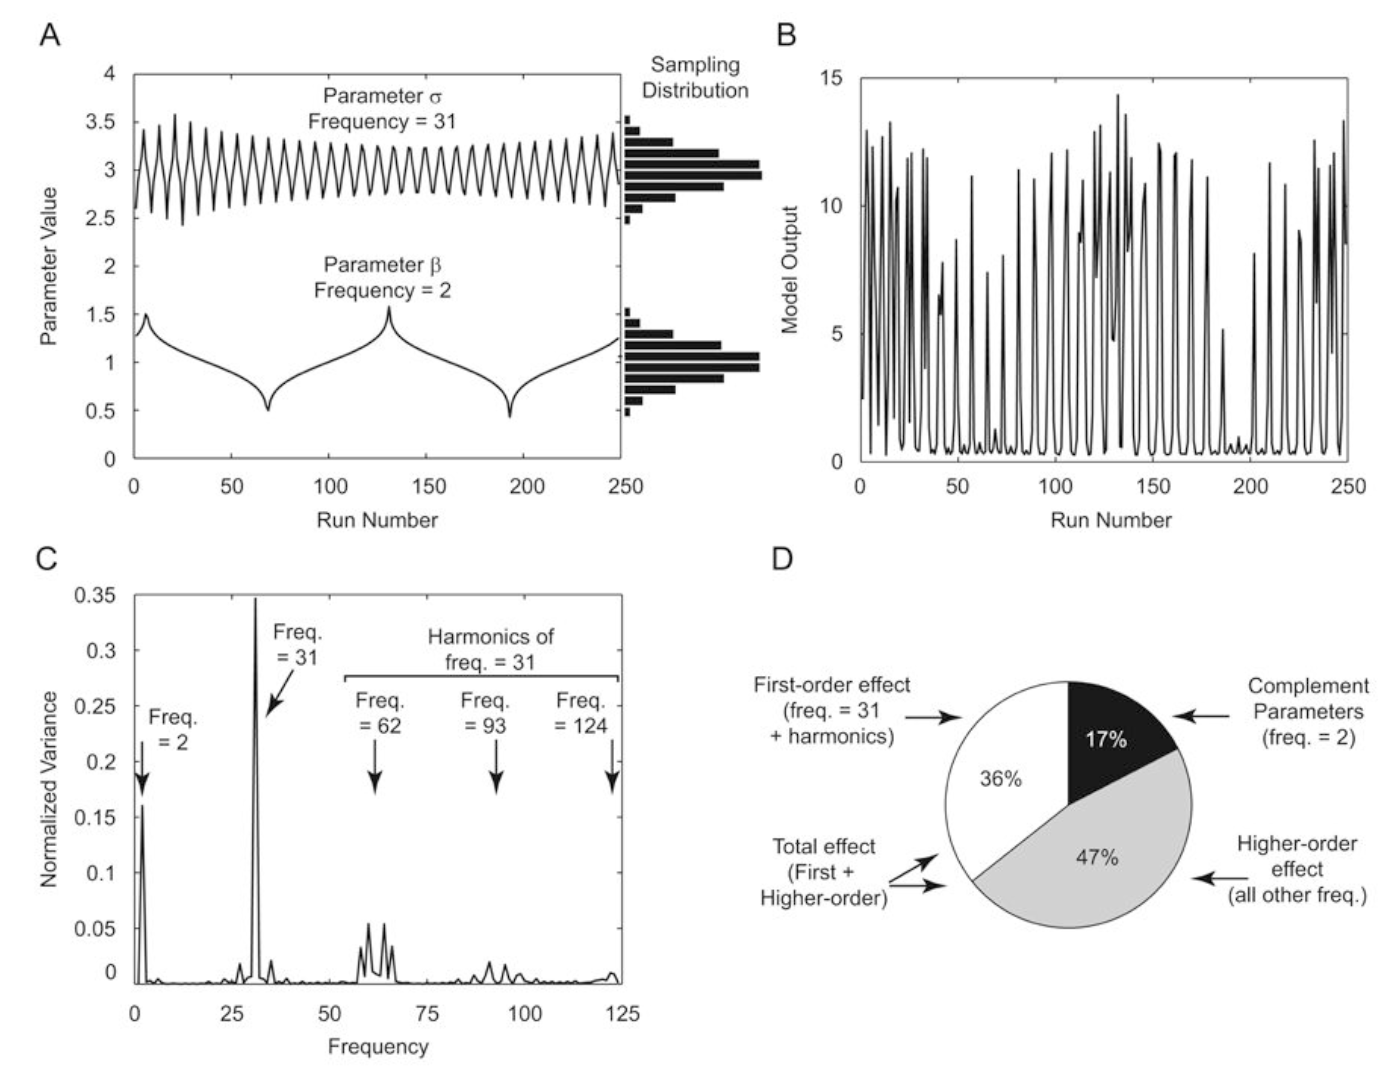
\includegraphics[width=0.7\textwidth]{images/FAST.png}
	\caption{eFAST analysis of the Lotka-Volterra model output. Reprinted from \cite{MARINO}.}
	\label{fig:FAST}
\end{figure}

\FloatBarrier

\section{Examples from cardiac modelling}

SA frameworks have shown to be useful in helping researchers better understand the inner structure of the models for knowledge discovery and predictive modelling, with extensive applications in numerous mathematical models in  different areas of study. In particular, the cardiac modelling field has seen extensive advancement over recent years thanks to the availability of experimental data, and the development of tools for solving differential equations in models of heart mechanics and electrophysiology (EP).  Models of cardiac function have become multi-scale and highly complex in that they integrate models spanning different organizational levels, ranging from molecular (ion channels, and contractile machinery), to cellular, tissue and whole organ levels. Models of single cell function, for instance, can include dozens of differential equations coupled to several constitutive equations, and include over a hundred model parameters. These models have been widely used to advance our understanding of fundamental mechanisms of cardiac function and the pathophysiology of heart diseases, to develop novel treatment strategies, and surgical guidance.

Physiological variability in cardiac EP is linked to several factors, such as, the stochastic nature of ion channel gating, natural cell variability (variable cell size, ion channel expression, etc.), and the non-linear behaviour of AP restitution. These manifest in variable ion channel function, calcium signalling, and electrical propagation in the tissue.  Therefore, deterministic cardiac models that do not account for uncertainty in the parameters are prone to provide unreliable results and lead to misleading conclusions. Inherent uncertainties and variability should therefore be properly addressed to improve reliability of cardiac simulations and enable predictive modelling in clinical practice.
In that respect, interest in UQ and SA has grown among the cardiac modelling community over recent years, with the importance of handling uncertainties and variability in cardiac modelling being addressed by some authors \cite{HUBERTS201868,Mirams}. 

In this section I will present a few examples of how UQ ans SA has been applied in cardiac modelling to help answers question such as ``\textit{what are the most influential parameters in determining the observed mechanical and electrical behaviour of cardiac models?}'', ``\textit{what are the physiological ranges of parameters that result in a particular behaviour of interest?}', and ``\textit{how does the choice of parameters affect the predictions of the model?}'''. 

\vspace{0.5cm}
In the work of Hurtado et al. \cite{Hurtado}, the authors used PCE and the elementary effects method to perform forward uncertainty propagation and sensitivity analysis on two coupled models of excitation-contraction of a 3D model stripe of a cardiac tissue. The authors looked at how variability in maximal conductances of major ionic currents affect selected QOIs, such as the action potential duration (APD90), calcium transient amplitude (CaT), cardiac stretch, and mechanical stress. 
Their results suggested a linear relationship between maximal conductances and the quantities of interest for a variability in parameters up to 25\%. Therefore, the authors used linear response surfaces to compute the empirical probability density functions of model responses. 
They found that a larger variability of the model parameters resulted in a larger variability of the model outputs, as expected (Fig. \ref{fig:Hurtado1}). Furthermore, APD90 and CaT were mostly affected by the maximal conductances of L-type calcium current (ICaL), and the slow delayed rectifier potassium current (IKs), and that stretch and stress were mostly influenced by ICaL alone, as shown in Fig. \ref{fig:Hurtado2}. This suggested a poor mechanoelectric feedback in models of cardiac electromechanics.

%\begin{figure}[h]
%	\centering
%	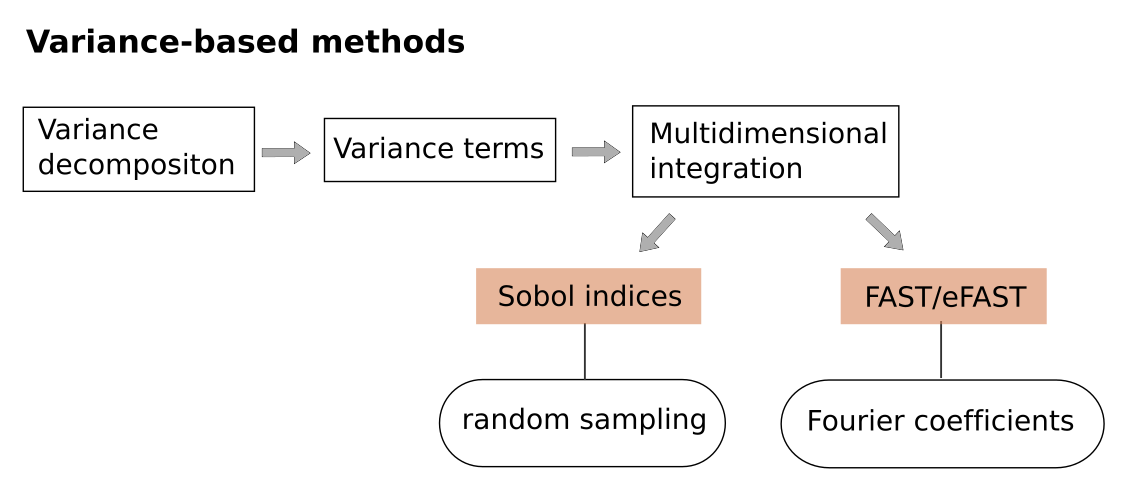
\includegraphics[width=0.7\textwidth]{images/variance_methods.png}
%	\caption{ Adapted from \cite{Hurtado}.}
%	\label{fig:variance_methods}
%\end{figure}

%\begin{figure}[h]
%	\centering
%	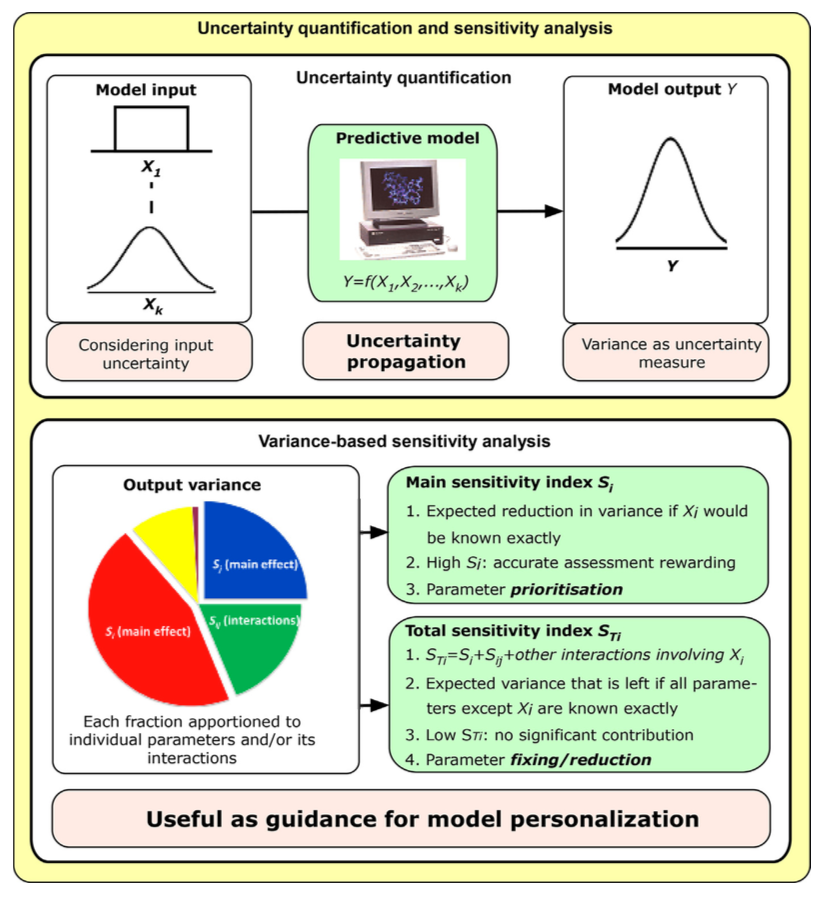
\includegraphics[width=0.7\textwidth]{images/personalization.png}
%	\caption{ Reprint from \cite{HUBERTS201868}.}
%	\label{fig:personalization}
%\end{figure}

\begin{figure}[h]
	\centering
	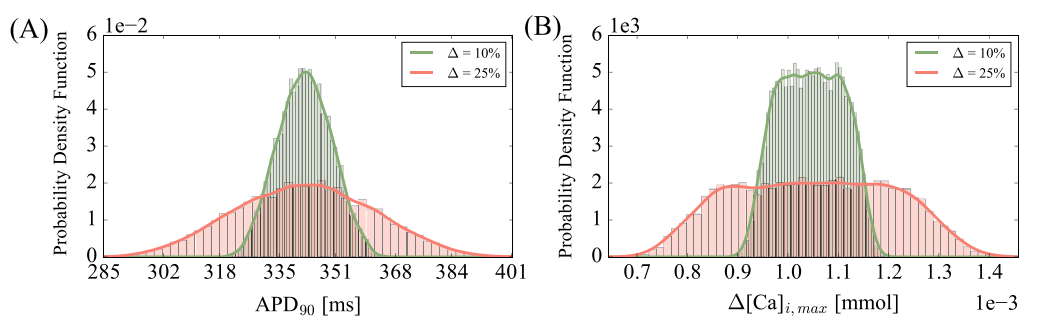
\includegraphics[width=0.9\textwidth]{images/Hurtado1.png}
	\caption{ Empirical probability density functiosn of the electromechanical model corresponding to 10\% and 25\% parameter variability for APD90 (A), and CaT ($\Delta[Ca]_{i, max}$) (B). Reprinted from \cite{Hurtado}.}
	\label{fig:Hurtado1}
\end{figure}

\begin{figure}[h]
	\centering
	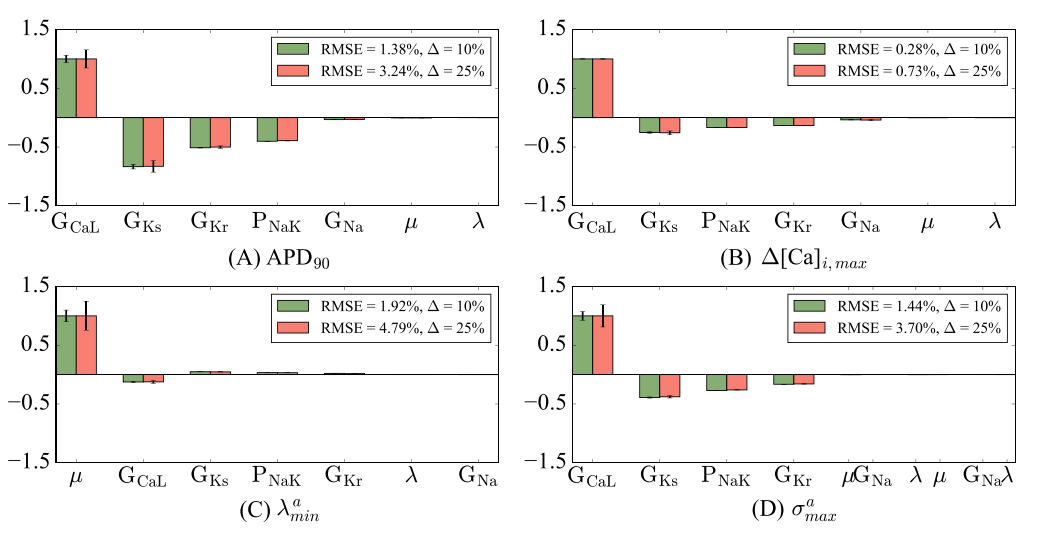
\includegraphics[width=0.9\textwidth]{images/Hurtado2.png}
	\caption{Parameter sensitivity measures $\mu^{*}$ (bar) and $\sigma^{*}$ (error bars) from elementary-effects analysis of the electromechanical model: APD90 (A),  CaT ($\Delta[Ca]_{i, max}$) (B), stretch ($\lambda_{a}$) (C), and stress ($\sigma_{a.max}$) (D). Reprinted from \cite{Hurtado}.}
	\label{fig:Hurtado2}
\end{figure}

\vspace{0.5cm}
Models of single cell EP have also been subjected to SA, mainly to help researchers dissect the role of the several model parameters in the action potential (AP) and calcium transient morphologies under a varied set of conditions. Furthermore, it has been observed that these models are degenerate in that different sets of model parameters can produce similar AP and CaT shapes (Fig. \ref{fig:AP_CaT}), and thus SA can help guide the best choice of parameter sets.  Examples in this area include the work of Sobie and Sarkar et al. \cite{SOBIE20091264,Sobie2010}, Britton et al. \cite{BrittonE2098}, and Sanchez et al. \cite{Sanchez}. In this approach, the authors used LHS to sample the parameter space, assuming a uniform distribution of the parameters, producing a large number of samples (up to 10.000). These samples are then used to perform an equal number of model evaluations to produce what is called \textit{population of models} (PoM). Each model in the PoM outputs a number of QOIs, typically being APD90, CaT, resting membrane potential, upstroke velocity, and CaT duration. Because all these quantities can be measured experimentally, the populations are subsequently \textit{experimentally calibrated} to eliminate unphysiological models from the subsequent analyses. Most commonly varied input parameters that are related to the ionic currents, and in particular, the maximal conductances since these are known to great affect the behaviour of EP models. The results of the model simulations are then linearly regressed onto the varied model parameters to obtain regression coefficients that can be used to rank the parameters in order of their importance, as shown in Fig. \ref{fig:Sobie}. 

Furthermore, output QOI can be used to segment calibrated PoM in accordance to distinguishable model behaviours, for instance APD90 above or below a certain threshold. This approach allows to test hypotheses related to the existence of significant differences in parameter distributions of both sub-populations. This analysis can provide useful insight into potential driving mechanisms of either behaviour. For instance, in \cite{Sanchez} the authors constructed two PoMs of atrial cell models for three different cell models - the Maleckar, Courtemanche, and Grandi models; one PoM consisting of normal cells, and the other consisting of a diseased phenotype (cAF) ,and then compared the parameter distributions underlying each of the experimentally calibrated PoMs, revealing some significant differences among the two groups of parameters (Fig. \ref{fig:Sanchez}), which can indicate the potential role of the underlying mechanisms in the development of the diseased phenotype .  

\begin{figure}[h]
	\centering
	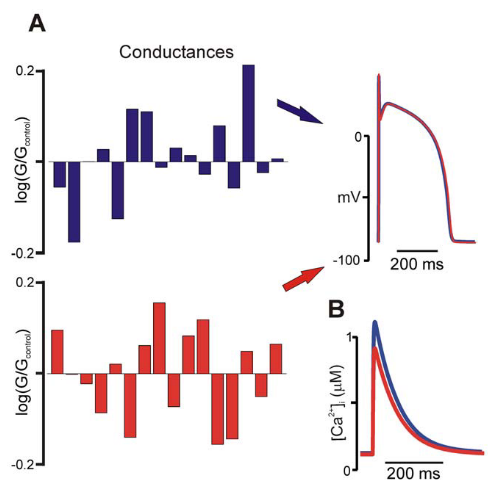
\includegraphics[width=0.4\textwidth]{images/AP_CaT.png}
	\caption{Non-uniqueness of EP model simulations, showing two different combinations of parameters of ionic conductances resulting in nearly identical action potential morphology (A).  However, intracellular calcium  transients produced by the same parameter combinations show some differences (B), suggesting that such information could be used to distinguish between the two parameter sets. Reprinted from \cite{Sobie2010}.}
	\label{fig:AP_CaT}
\end{figure}

\begin{figure}[h]
	\centering
	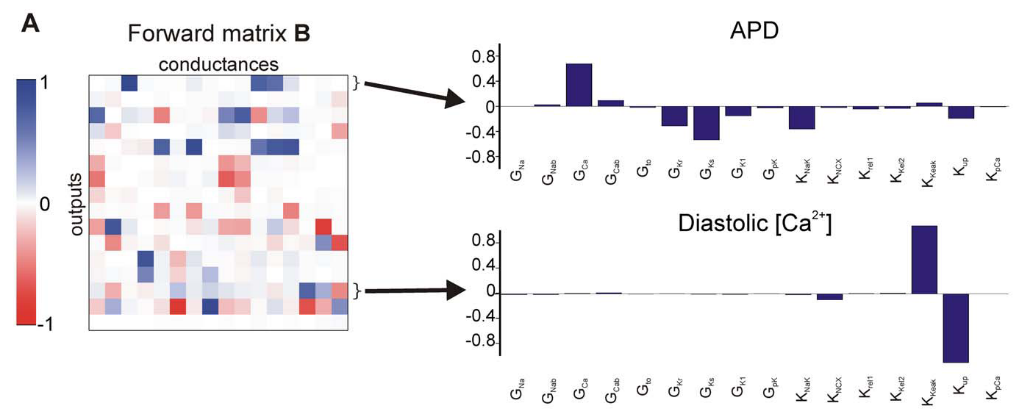
\includegraphics[width=0.8\textwidth]{images/Sobie.png}
	\caption{Parameter sensitivities obtained from regression analyses shown as ``heat maps'',  with white representing values near zeros, and blue and red indicating positive and negative values, respectively. Each row of the forward matrix \textbf{B} represents the contributions of each of the conductances to a particular output, with APD and CaT shown in bar graphs to the right. Reprinted from \cite{Sobie2010}.}
	\label{fig:Sobie}
\end{figure}

\begin{figure}
	\centering
	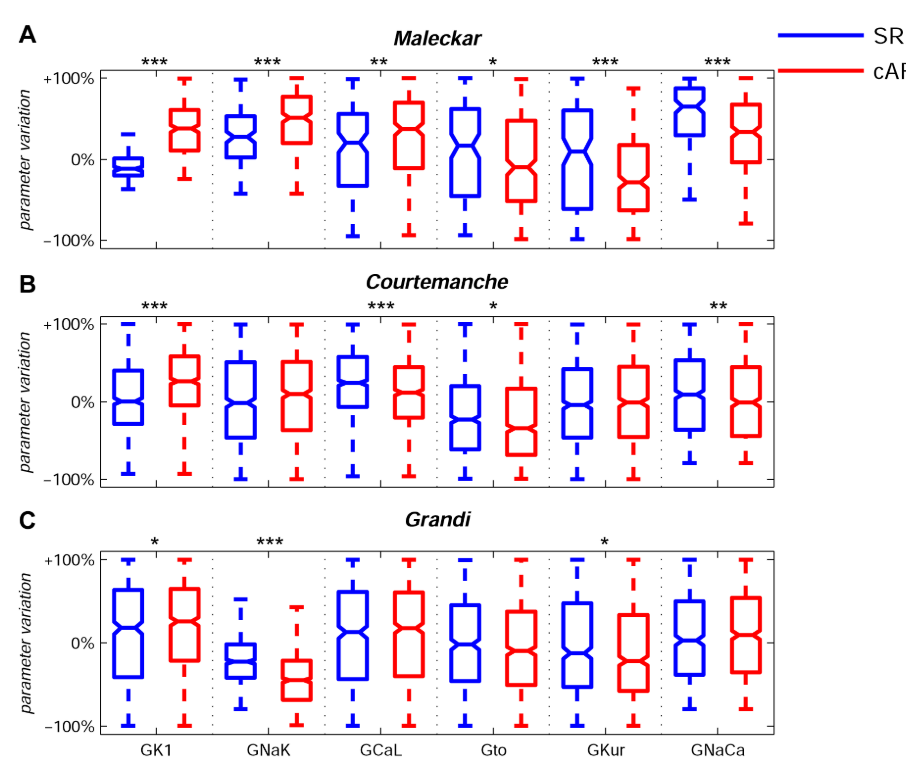
\includegraphics[width=0.5\textwidth]{images/Sanchez.png}
	\caption{Boxplots showing the ranges of variability of ionic conductances of two distinct populations of models obtained with three different human atrial AP models: Maleckar (A), Courtemanche (B) and Grandi (C) human atria AP models. The distinct populations correspond to in normal cells (blue) and diseased cells (red). Each boxplot represents the range covered by the ionic conductances. Reprinted from \cite{Sanchez}. }
	\label{fig:Sanchez}
\end{figure}

\vspace{0.5cm}
In \cite{Romero2009}, Romero et al. performed local SA in a model the human ventricular cellular electrophysiology to investigate how natural variability or drug-induced alterations in ionic current properties are related to arrhythmic risk. The authors varied the maximal conductances and time constants of the main transmembrane ionic currents involved in AP repolarization, one parameter at a time by by -30\% and -15\%, +15\% and +30\%. Although performed as a local method, the analysis in this study provided some insights into the relative importance of the varied parameters to action potential properties, calcium and sodium dynamics, as well as their rate dependence.

In another example, Hu et al. \cite{HU201857} used the generalised PCE framework to perform forward UQ on multi-scale models of cardiac tissue with parametric uncertainty at the ion channel and cell levels. They looked at the effect of inserting uncertainties in several parameters related to two potassium channel on several multi-scale model outputs, such as steady state activation and inactivation of ion channels, AP duration, conduction velocity and spiral wave dynamics. Additionally, they performed variance-based SA with MC sampling to uncover the relevant parameters for these model responses in order to select which parameters to consider for uncertainty propagation. They also compared the accuracy and computational burden of the PCE method as compared to performing MC simulations, concluding that PCE was an much more effective method for computing parameters of the uncertainty distributions of the outputs (mean and variance), requiring only a fraction of the computational time required by using MC with 10.000 samples, while achieving comparable accuracy. As an example, Fig. \ref{fig:Hu} shows the uncertainty in steady state activation and inactivation of IKto with 5\% and 10\% parameter variability achieved with both the PCE and MC methods. 

\begin{figure}
	\centering
	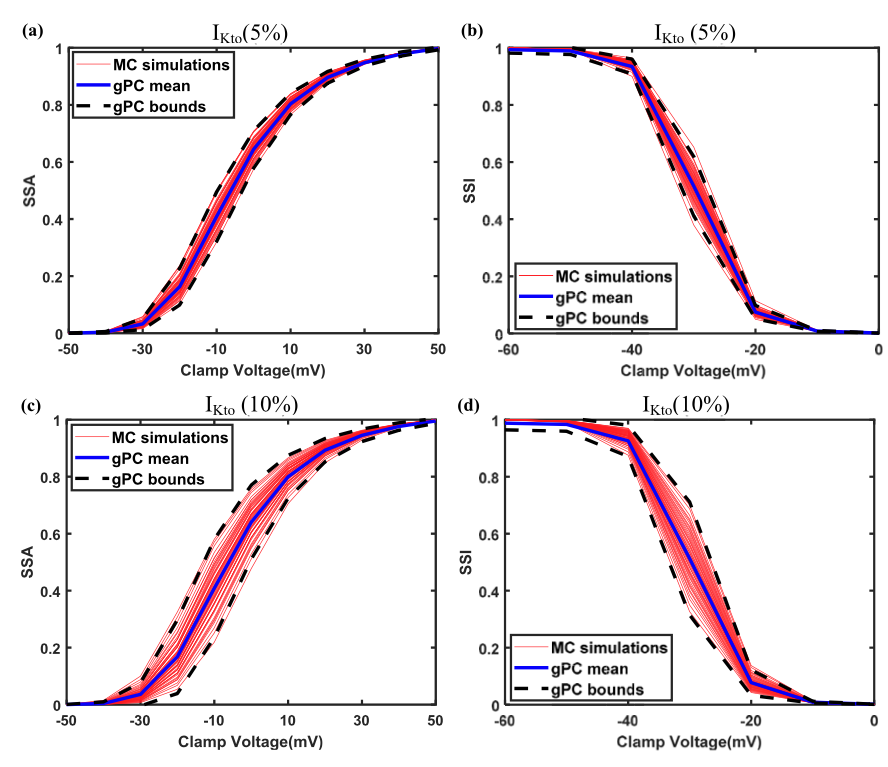
\includegraphics[width=0.5\textwidth]{images/Hu.png}
	\caption{Comparison between the PCE method and MC simulation. (a) and (c) show the upper and lower bounds of the steady state activation curve of IKto, and (b) and (c) show the upper and lower bounds of the steady state inactivation curve of IKto. Reprinted from \cite{HU201857}.}
	\label{fig:Hu}
\end{figure}

\FloatBarrier

\section{Synthesis and conclusions}

The present essay aimed at providing an overview of some of the most commonly used uncertainty quantification and sensitivity analysis techniques.  The extensive existing literature on UQ and SA, both regarding the development of methods and application to numerous real problems, is more than a convincing indicator of usefulness and applicability of these techniques. Therefore, an exhaustive review of the literature was out of the scope of this work. However, the methods presented here were selected so as to provide a wide enough range of different approaches and applicabilities.  

The SA methods presented in this essay, although similar in some aspects, do not provide exactly the same information. Therefore, in certain instances it may be advantageous to perform more than one analysis, for instance, correlation and variance decomposition, in order to gain more insight into the sensitivities of the model. Furthermore, the availability of SA methods is vast and the choice of best method can become difficult. Some authors have to reviewed the different SA methods, with the assumptions and applications implicit to each one of them, in an attempt to provide some guidance in choosing the SA method for the particular model at hand. A few examples of such synthesis are presented in Fig. \ref{fig:SA_method_chart} and \ref{fig:SA_method_selection} below. 

\begin{figure}[!ht]
	\centering
	\caption{Table comparing different SA methods based on several comparison criteria. Reprint from \cite{iooss:hal-00975701}.}
	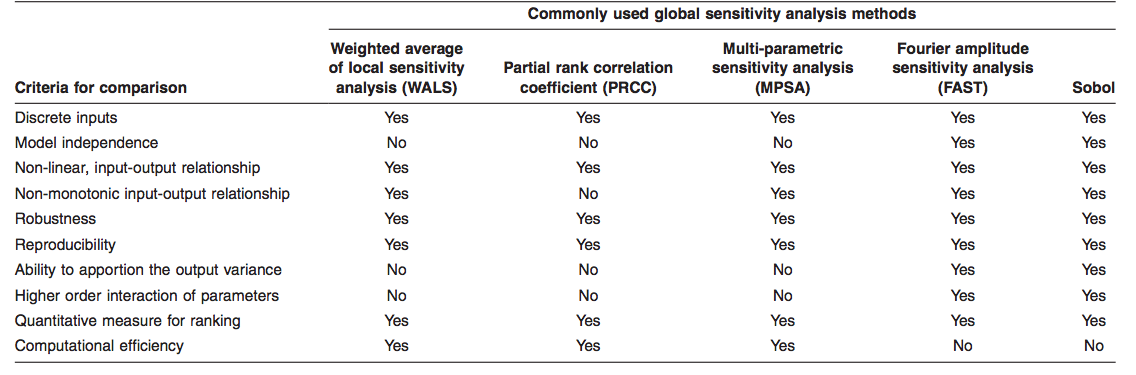
\includegraphics[width=1\textwidth]{images/SA_methods_table.png}
	\label{fig:SA_methods_table}
\end{figure}

\begin{figure}[!ht]
	\centering
	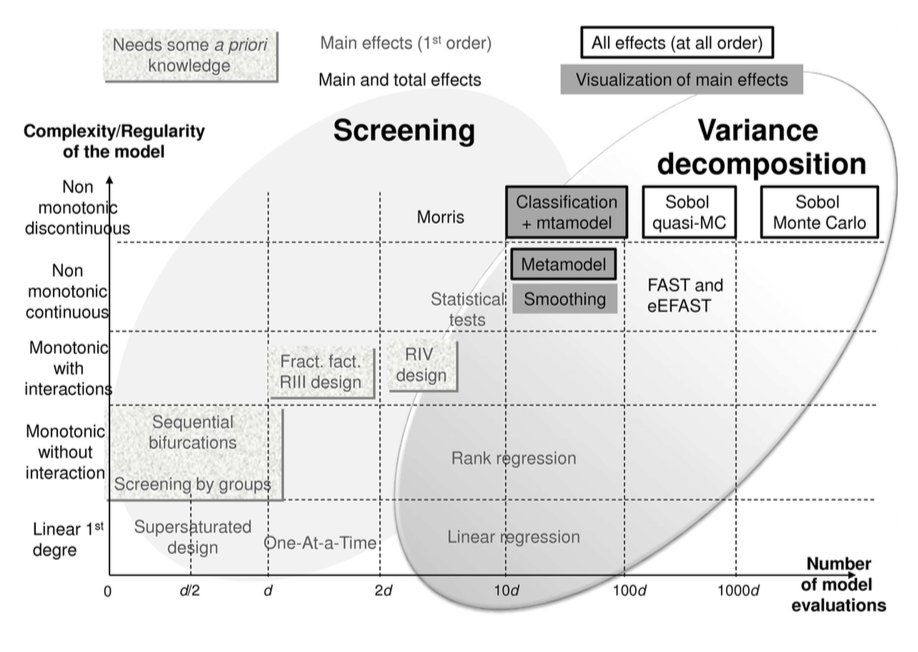
\includegraphics[width=0.85\textwidth]{images/SA_method_chart.png}
	\caption{A graphical representation of different SA methods comparing their performance in terms of number of model evaluations required for different types of models. Reprint from \cite{iooss:hal-00975701}.}
	\label{fig:SA_method_chart}
\end{figure}

\begin{figure}[!ht]
	\centering
	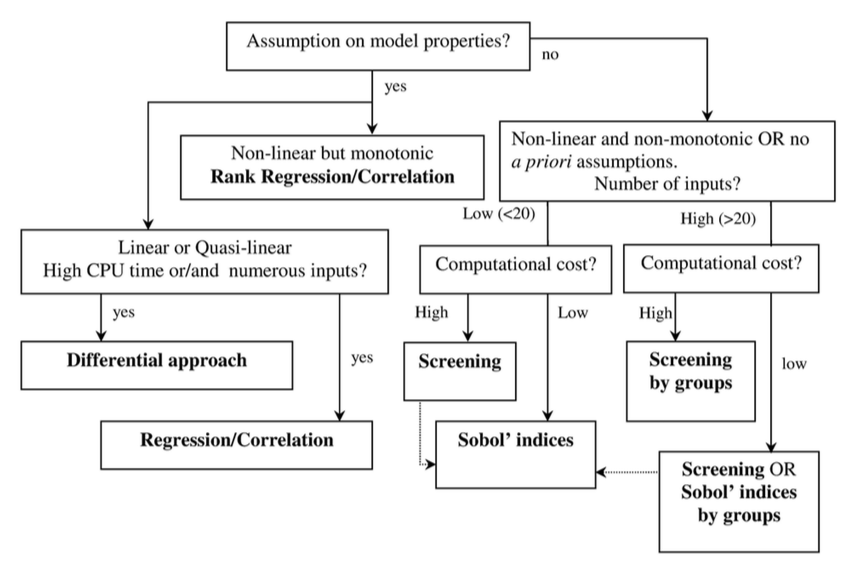
\includegraphics[width=0.85\textwidth]{images/SA_method_selection.png}
	\caption{Decision diagram for choosing the most appropriate SA method based on type of model, and computational cost.  Reprint from \cite{Rocquigny}.}
	\label{fig:SA_method_selection}
\end{figure}

\begin{figure}[!ht]
	\centering
	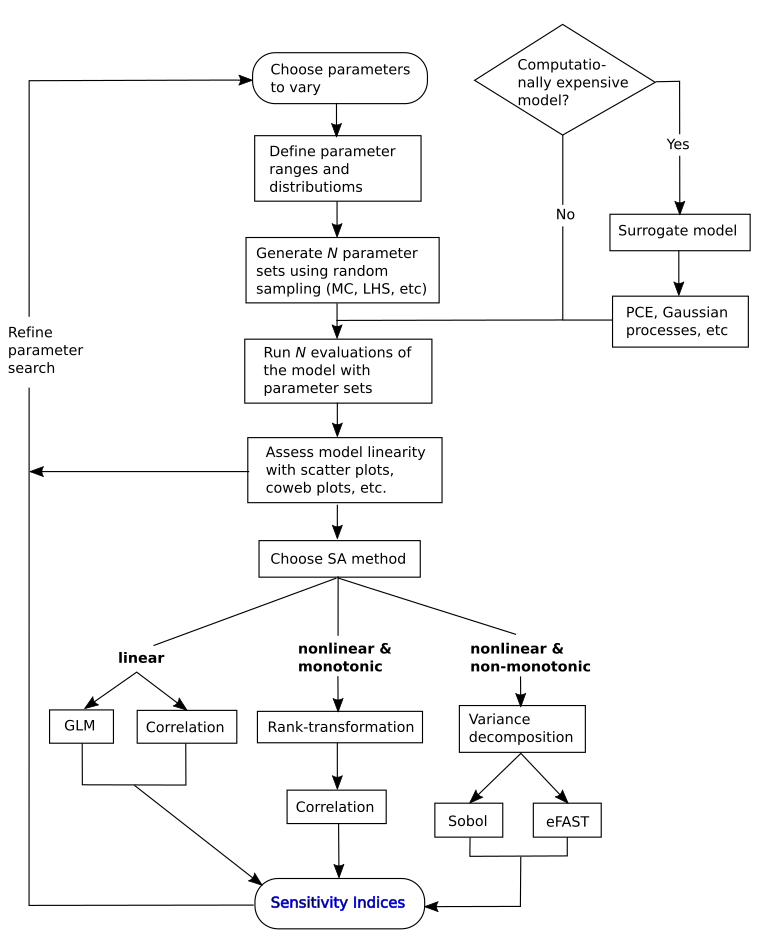
\includegraphics[width=0.85\textwidth]{images/SA_framework.png}
	\caption{A flow diagram of the general SA framework.}
	\label{fig:SA_framework}
\end{figure}

Sensitivity analysis is an growing field of study, and its importance is becoming ever more evident with the increasing use of computational modelling in several different areas. In the field of cardiac modelling in particular, modellers are increasingly recognizing the importance of acknowledging the uncertainty and variability in model, and thus more and more UQ and SA are being included in  model development routines.
It is important to for modellers to have a level of understanding of how variability and uncertainty affect the model predictions and confidence in the results. Although it is not yet standard routine, the development of UQ and SA tools will potentially facilitate the adoption of these techniques in a wider setting of model developers, and with that contribute to more accurate and reliable computational models. The present essay aimed at giving a small step towards disseminating the knowledge  of UQ and SA among non-experts. 

\FloatBarrier

\newpage
\bibliography{references}

\end{document}
